\documentclass[12pt,a4paper]{article}
\usepackage{fullpage}
\usepackage[margin=2cm]{geometry}
\usepackage{amsmath}
\usepackage{subfig}
\usepackage{graphicx}
\usepackage{caption}
\begin{document}
\title{Morphometry landmarks detection by convolutional neural network}
\author{LE Van Linh and BEURTON-AIMAR Marie}
\date{September, 2017}
\maketitle
\begin{abstract}

	In this work, we study the two methods that used to detect the landmarks on 2D images: \textbf{Deep Convolutional Network Cascade for Facial Point Detection} proposed by Yi Sun et al\cite{sun2013deep} and \textbf{Automatic ear detection and feature extraction using Geometric Morphometrics and Convolutional neural networks} from Celia Cintas et al\cite{cintas2016automatic}. Both articles have shown the convolution neural network (CNN) to study the landmarks on 2D images: Yi Sun studied the human face while Celia worked on human ears. Then, we show the results when applying the methods on pronotum of beetle. Finally, we propose a specific network to work on pronotum and compare the results.
\end{abstract}
\section{Model 1: Facial point detection by CNN}
Yi Sun et al\cite{sun2013deep} focused on five facial keypoints: \textit{left eye center}(LE), \textit{right eye center}(RE), \textit{nose tip}(N), \textit{left mouth corner}(LM) and \textit{right mouth corner}(RM) (called landmarks). A model with 3-levels of networks are proposed to study from high-level to low-level of the landmarks.
\subsection{Data}
The dataset with 13466 face images includes 5590 images from LFW \cite{huang2007labeled} and remaining images are downloaded from the web. The dataset is randomly divided into the training set with 10000 images and validation set with 33466 images. Each face is labeled with five landmarks and the bounding box is created around the face.
\subsection{Architecture}
The proposed architecture includes 3-levels of CNN: three networks at the first level, and ten networks for each remaining level(Fig.\ref{3levels}). The networks at level 1 is designed to detect multiple landmarks while two last levels are designed for working on each landmark.
\begin{figure}[h]
	\centering
	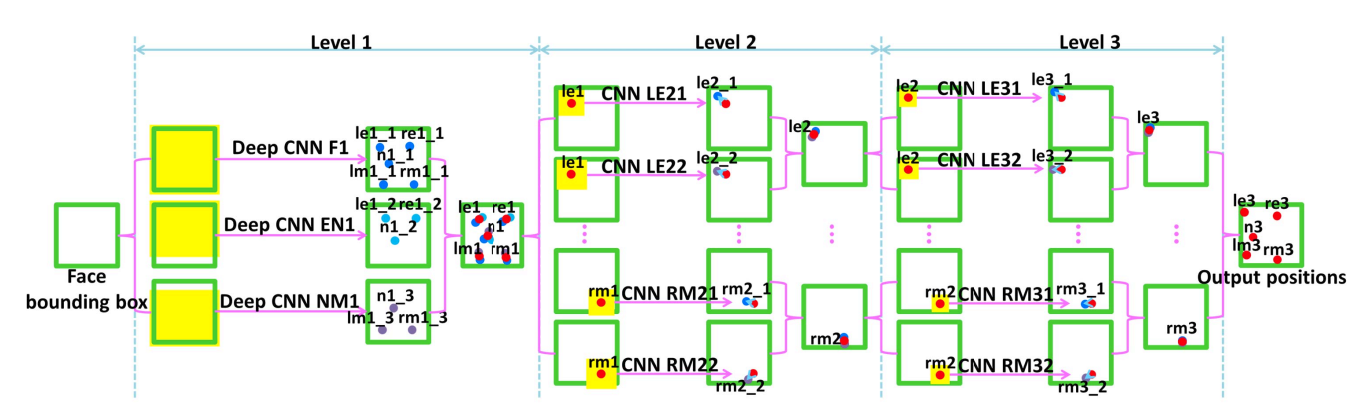
\includegraphics[scale=0.35]{images/3levels}
	\caption{The 3-levels proposed architecture}
	\label{3levels}
\end{figure}

At the first level, three CNNs are employed to study the location of the facial points: F1, EN1, NM1 whose input regions cover the whole face(size of $39 \times 39$). F1 is studied all the position of five landmarks; EN1 is worked on the eyes and nose while NM1 worked on nose and the mouth corners. Each network predicts the landmarks corresponding with the region that it covers. At the end of level 1, the coordinate of each landmark is averaged of coordinates that predicted from three networks. Fig.\ref{1Fconv} illustrates the deep structure of the networks at level 1, which contains four convolutional layers followed by max pooling and two dense layers. F1, EN1, and NM1 take the same structure but with different size of the input ($39 \times 31$) and different output at full-connected layers to suitable with the number of predicted landmarks.
\begin{figure}[h]
	\centering
	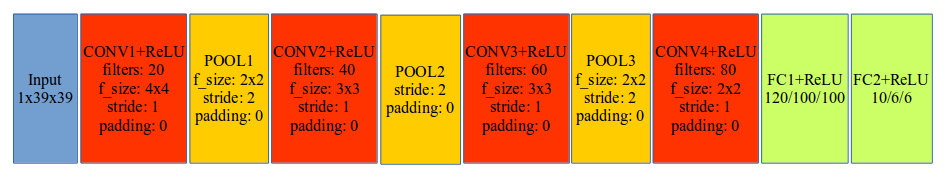
\includegraphics[scale=0.5]{images/cnn_level1}
	\caption{The structure of the networks in level 1}
	\label{1Fconv}
\end{figure}

The networks at the second and third levels take local patches centered at the predicted position of previous levels as input. Besides, they allowed to make small changes to previous prediction. The size of patches are also reduced along with the cascade model. For each position, two networks are used to predict the new positions. The last predicted position is average of the new positions. Fig.\ref{2lvconv} illustrates the architecture of the networks in level 2 and level 3. Basically, the networks in last two levels are similar, the only difference is the way to choose the patch around the landmark. A padding is added to the coordinates of the landmark to make the change of the patches i.e $0.16, 0.18$ in level 2 and $0.11, 0.12$ in level 3. Then, the patch is resized to the size of $15 \times 15$ before giving the networks.
\begin{figure}[h]
	\centering
	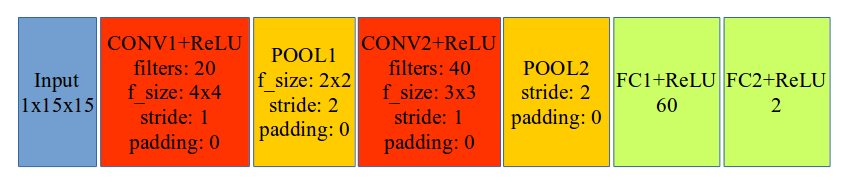
\includegraphics[scale=0.5]{images/cnn_level2}
	\caption{The structure of the networks in level 2, level 3}
	\label{2lvconv}
\end{figure}

 With 3-levels model, the purpose of the networks at the first level are estimated the landmark positions with large errors; the networks at last two levels are designed to achieve high accuracy.
\subsection{Experiments}
\subsubsection{Training}
At the first level, the patches according the bounding boxes (size of $39 \times 39$) are used as the input of the networks. At the following levels, the patches centered at previous predicted position is used to train. The size of the patches is decreased for each level. The learnable parameters include weight w, the gain g and the bias b which are initialized by small random number and learned by stochastic gradient descent.

The detection error on each facial point is measured by Eq.\ref{eq1}. If the error is greater than $5\%$, it is considered as failure.
\begin{equation}
	err = \sqrt{(x-x')^2 + (y-y')^2}/l
	\label{eq1}
\end{equation}
Where:
\begin{itemize}
	\item l is the width of the bounding box around the face.
	\item $(x,y)$ is ground truth facial point
	\item $(x',y')$ is predicted position
\end{itemize}
\subsubsection{Testing}
The model is tested with a dataset of 2557 face images. The image with the bounding box of the face is used as the input of the model. At the end, the predicted position is estimated from the model. By using the way in Eq.(\ref{eq1}) to evaluate the model, the error statistic on each level is obtained (Figs. \ref{rslevel1}, \ref{rslevel2}, \ref{rslevel3}).
%\begin{table}[h!]
%	\centering
%	\begin{tabular}{c}
%	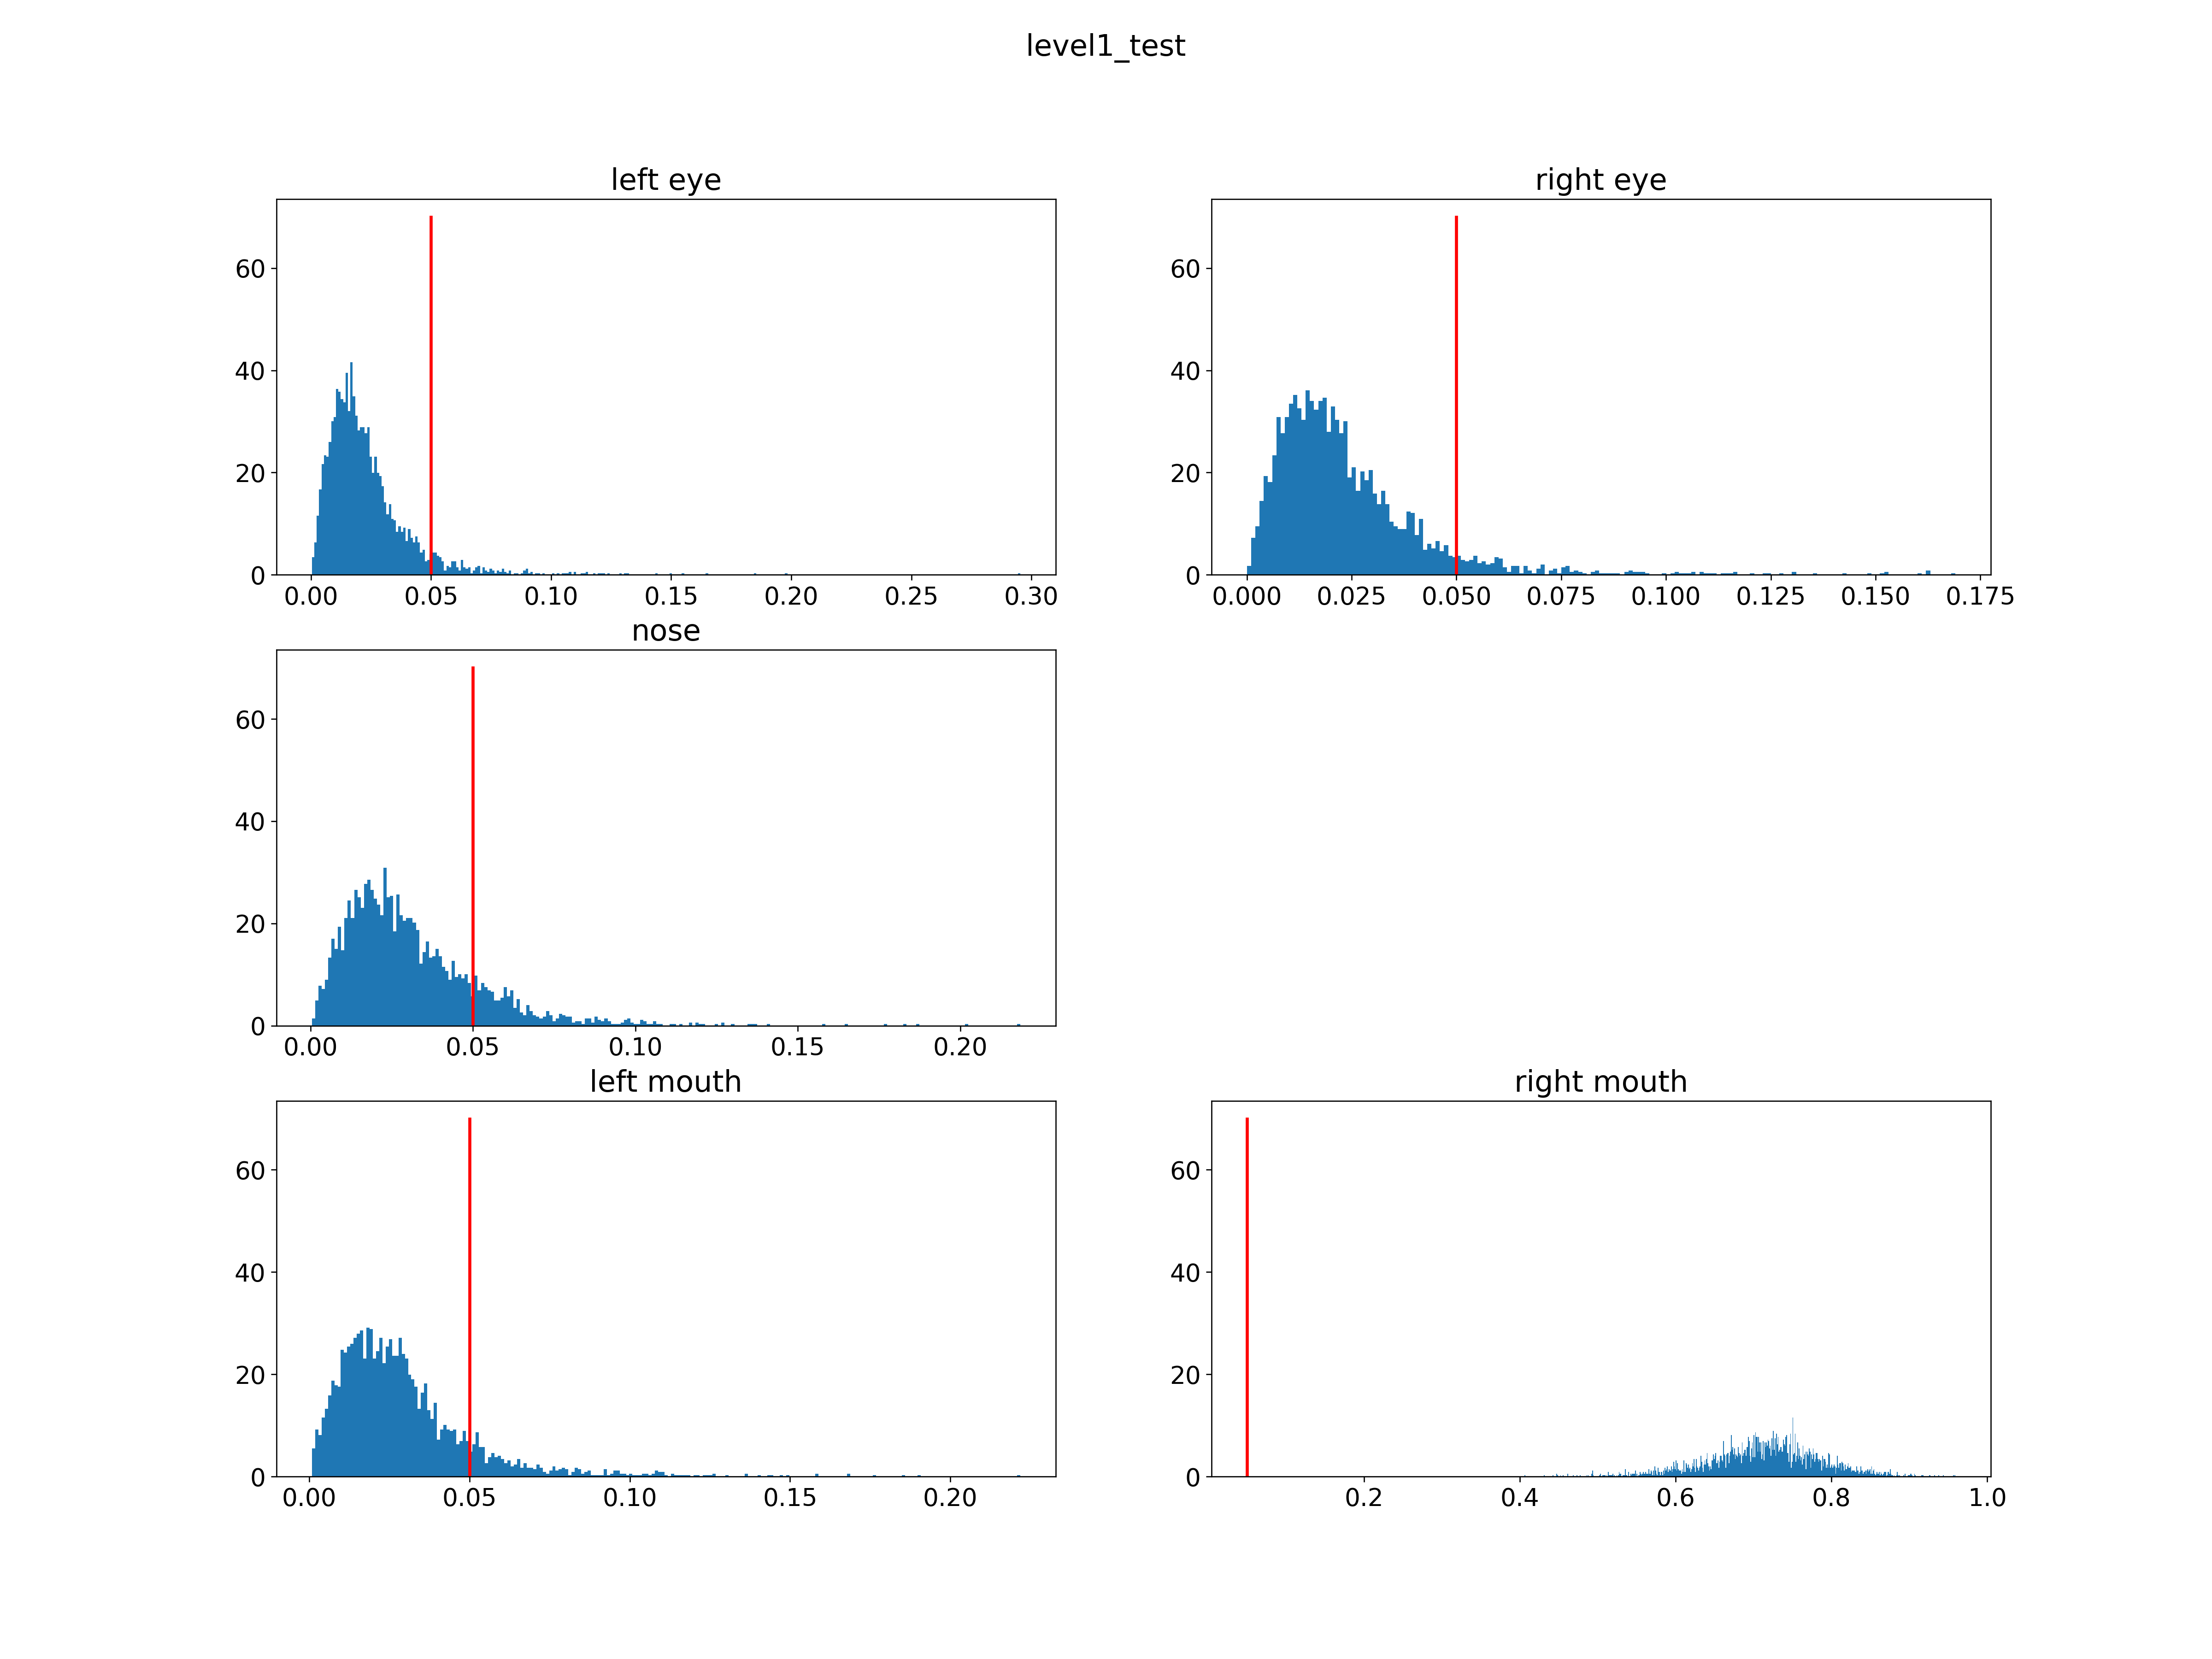
\includegraphics[scale=0.3]{images/level1_test}~\\
%	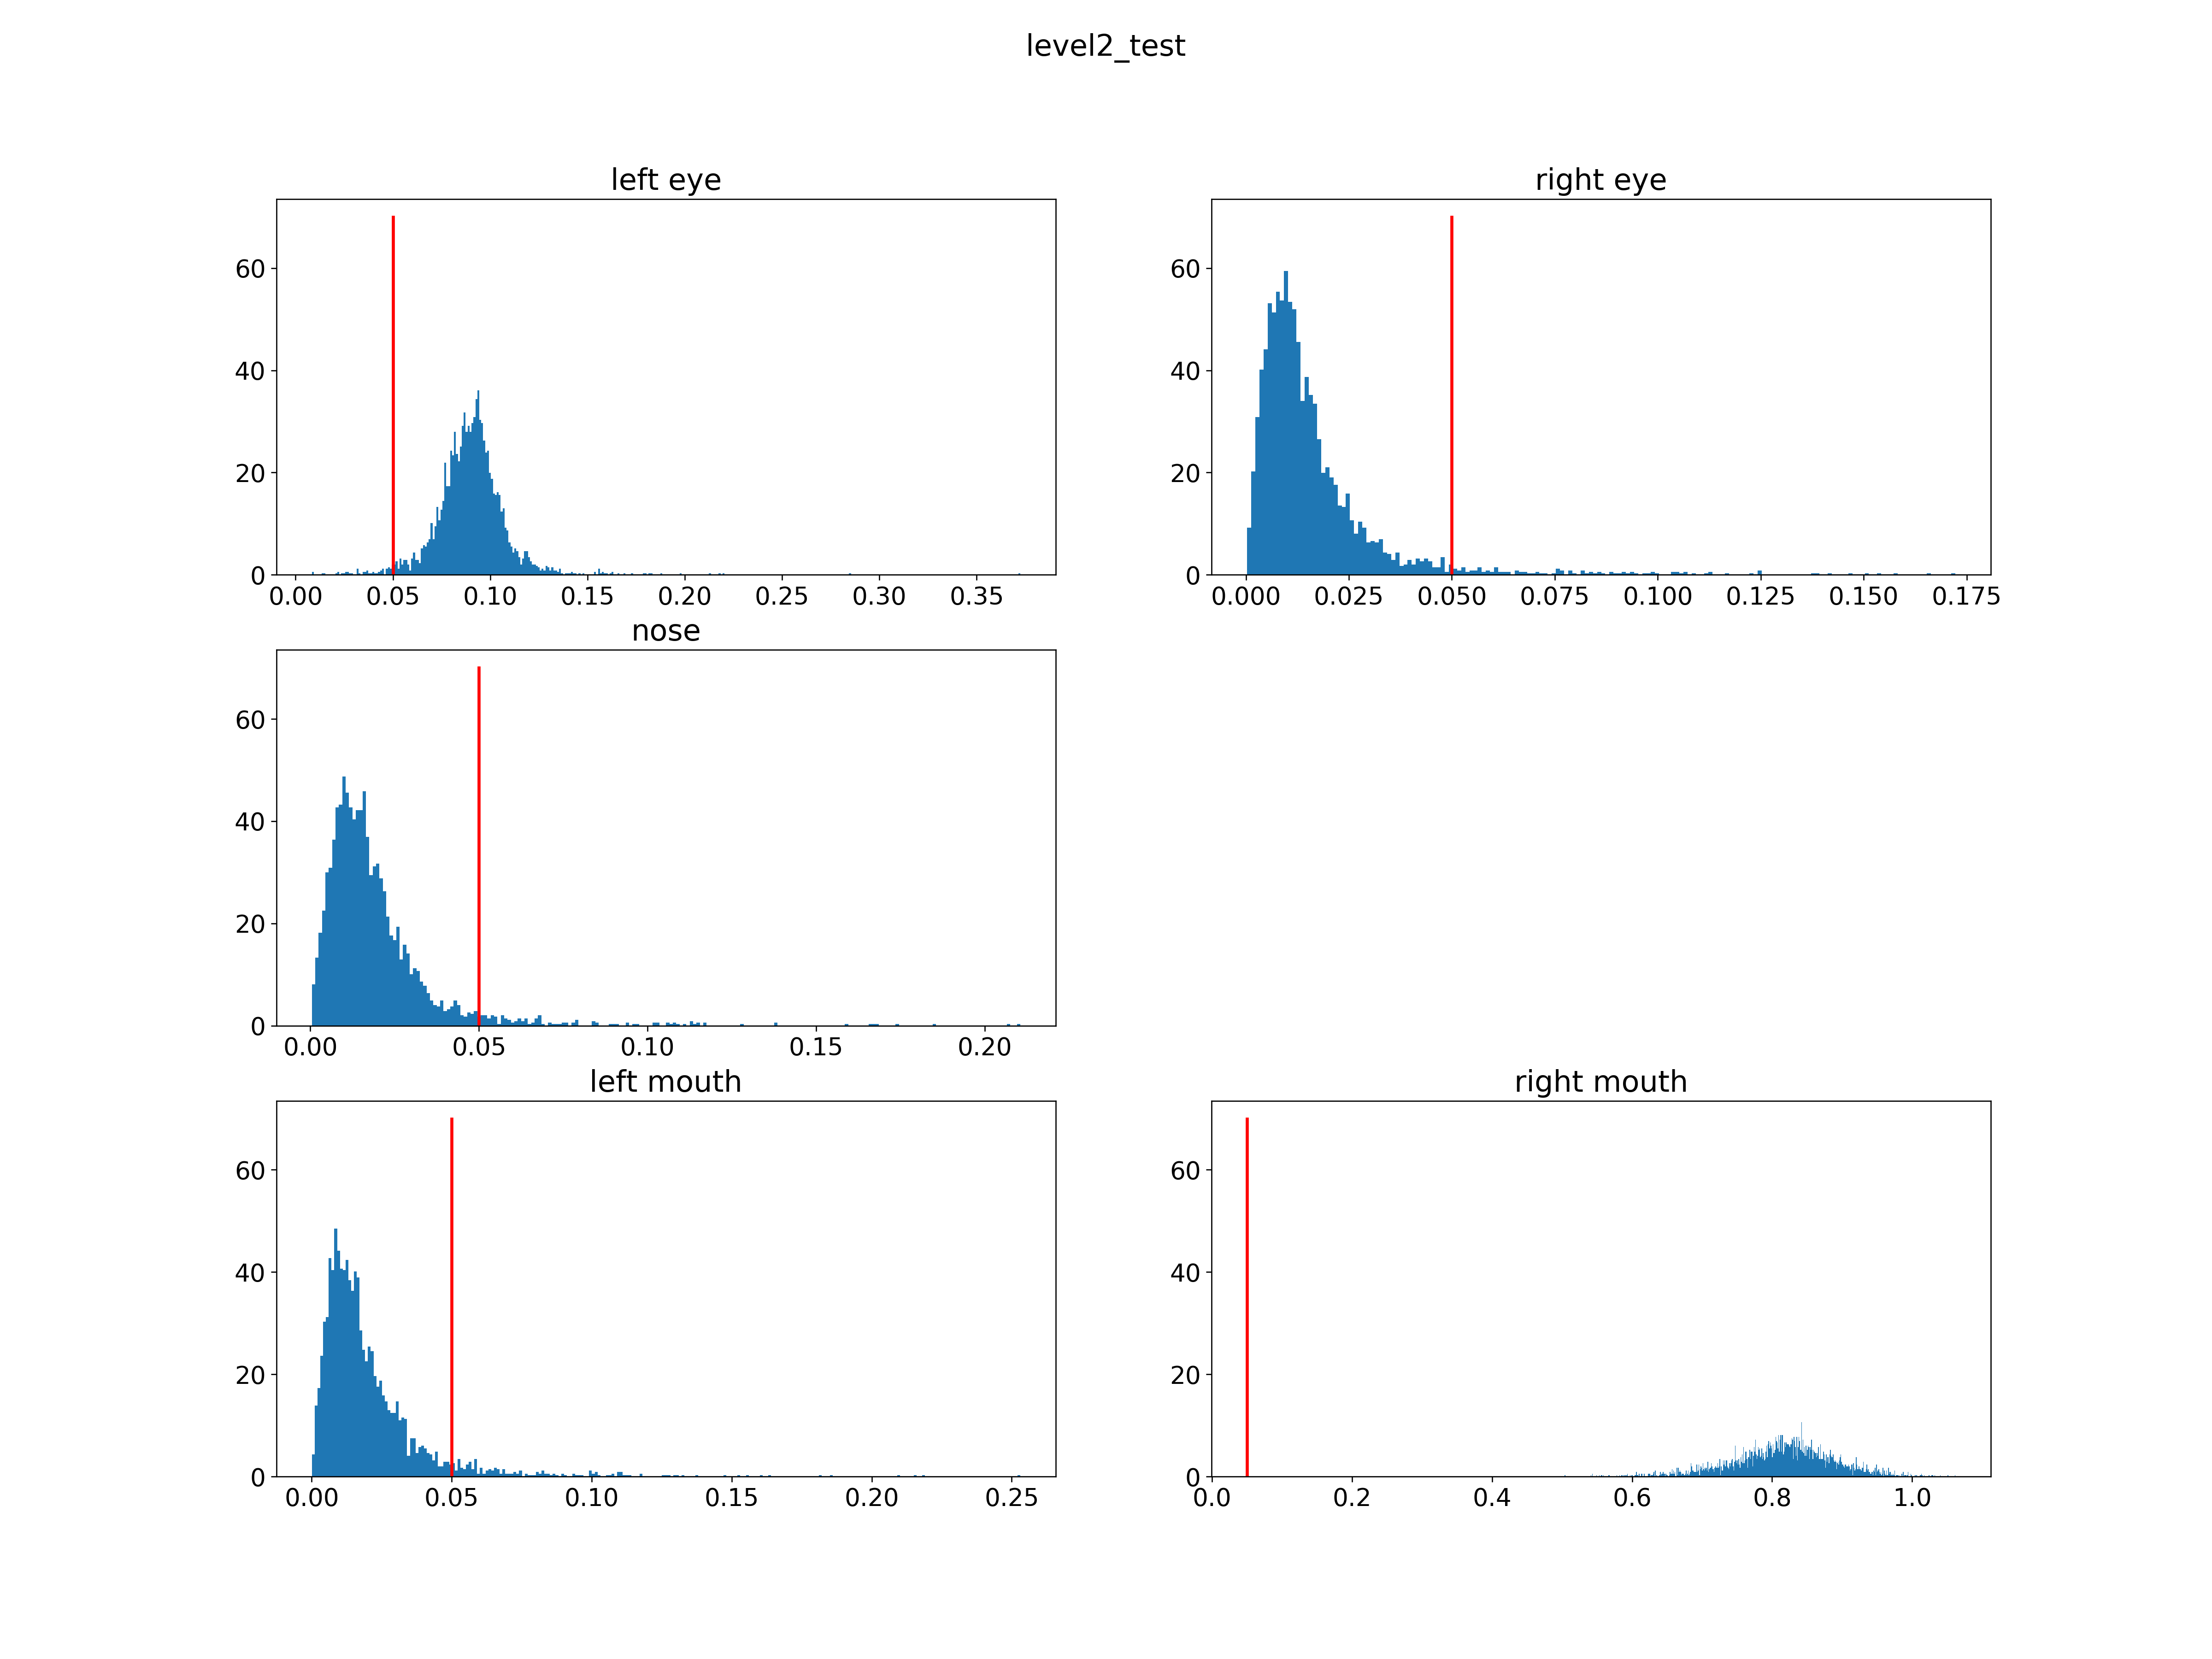
\includegraphics[scale=0.3]{images/level2_test}~\\
%	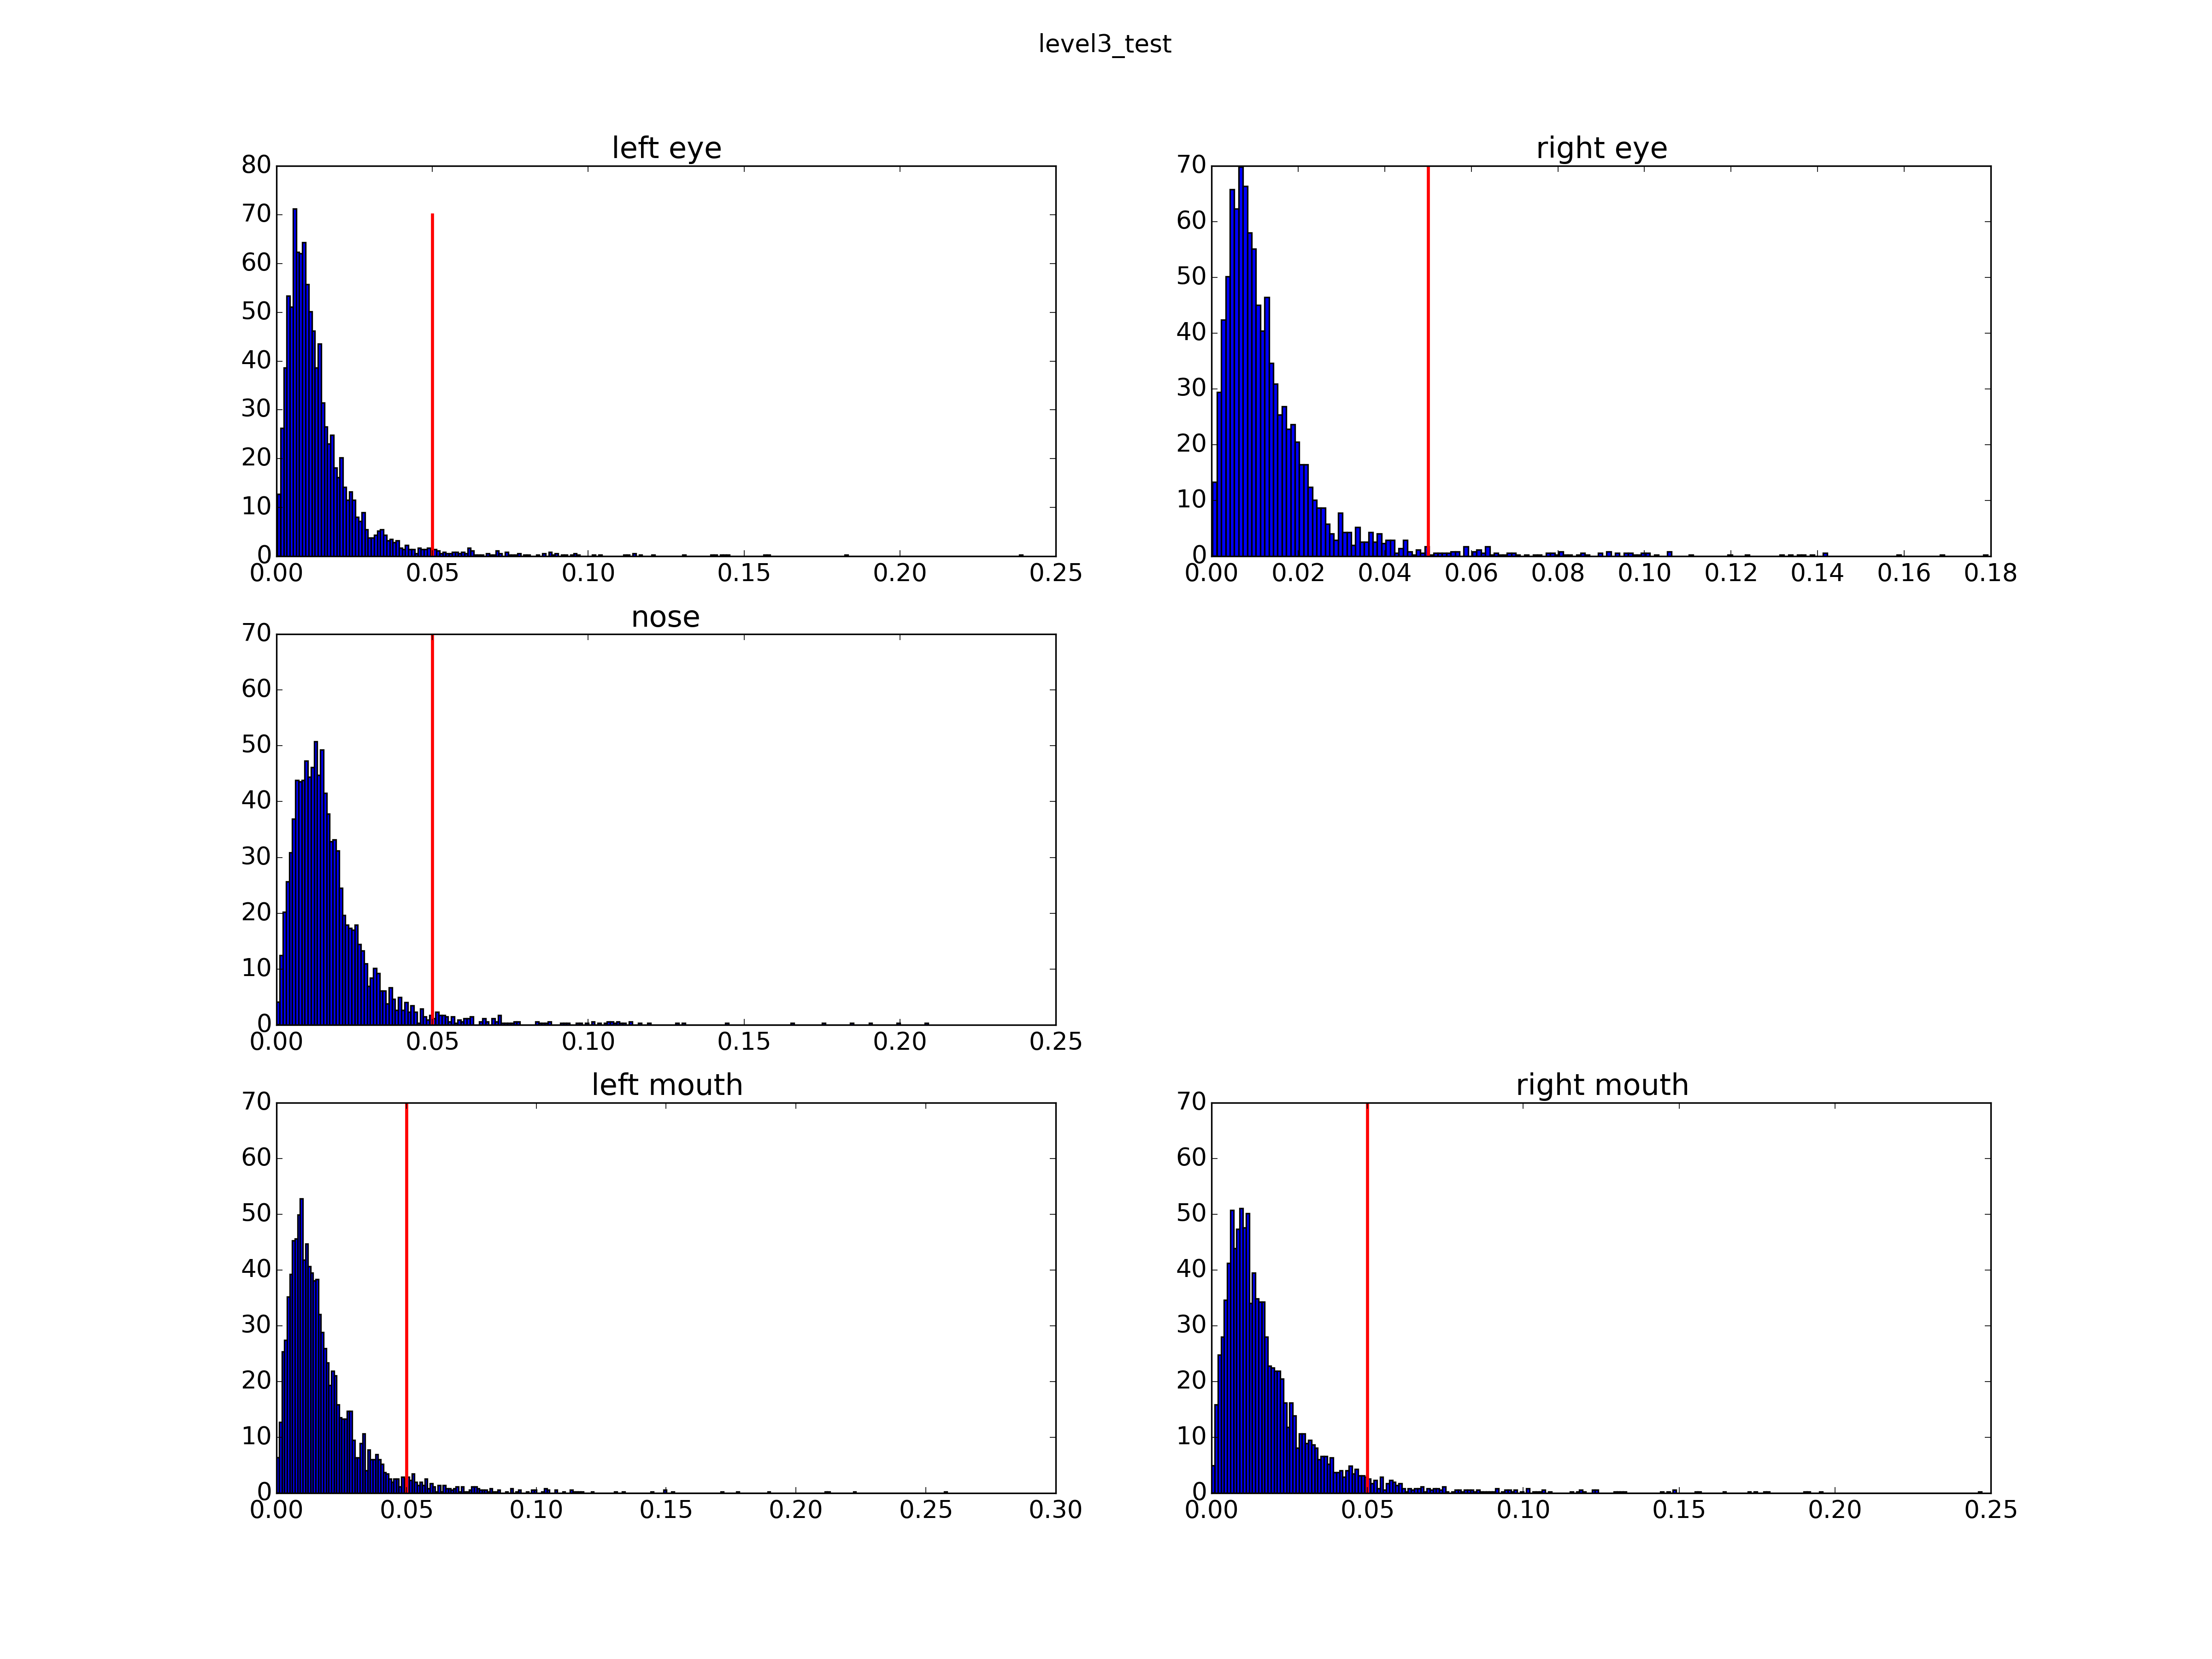
\includegraphics[scale=0.3]{images/level3_test}
%	\end{tabular}	
%\end{table}
\begin{figure}[h!]
	\centering
	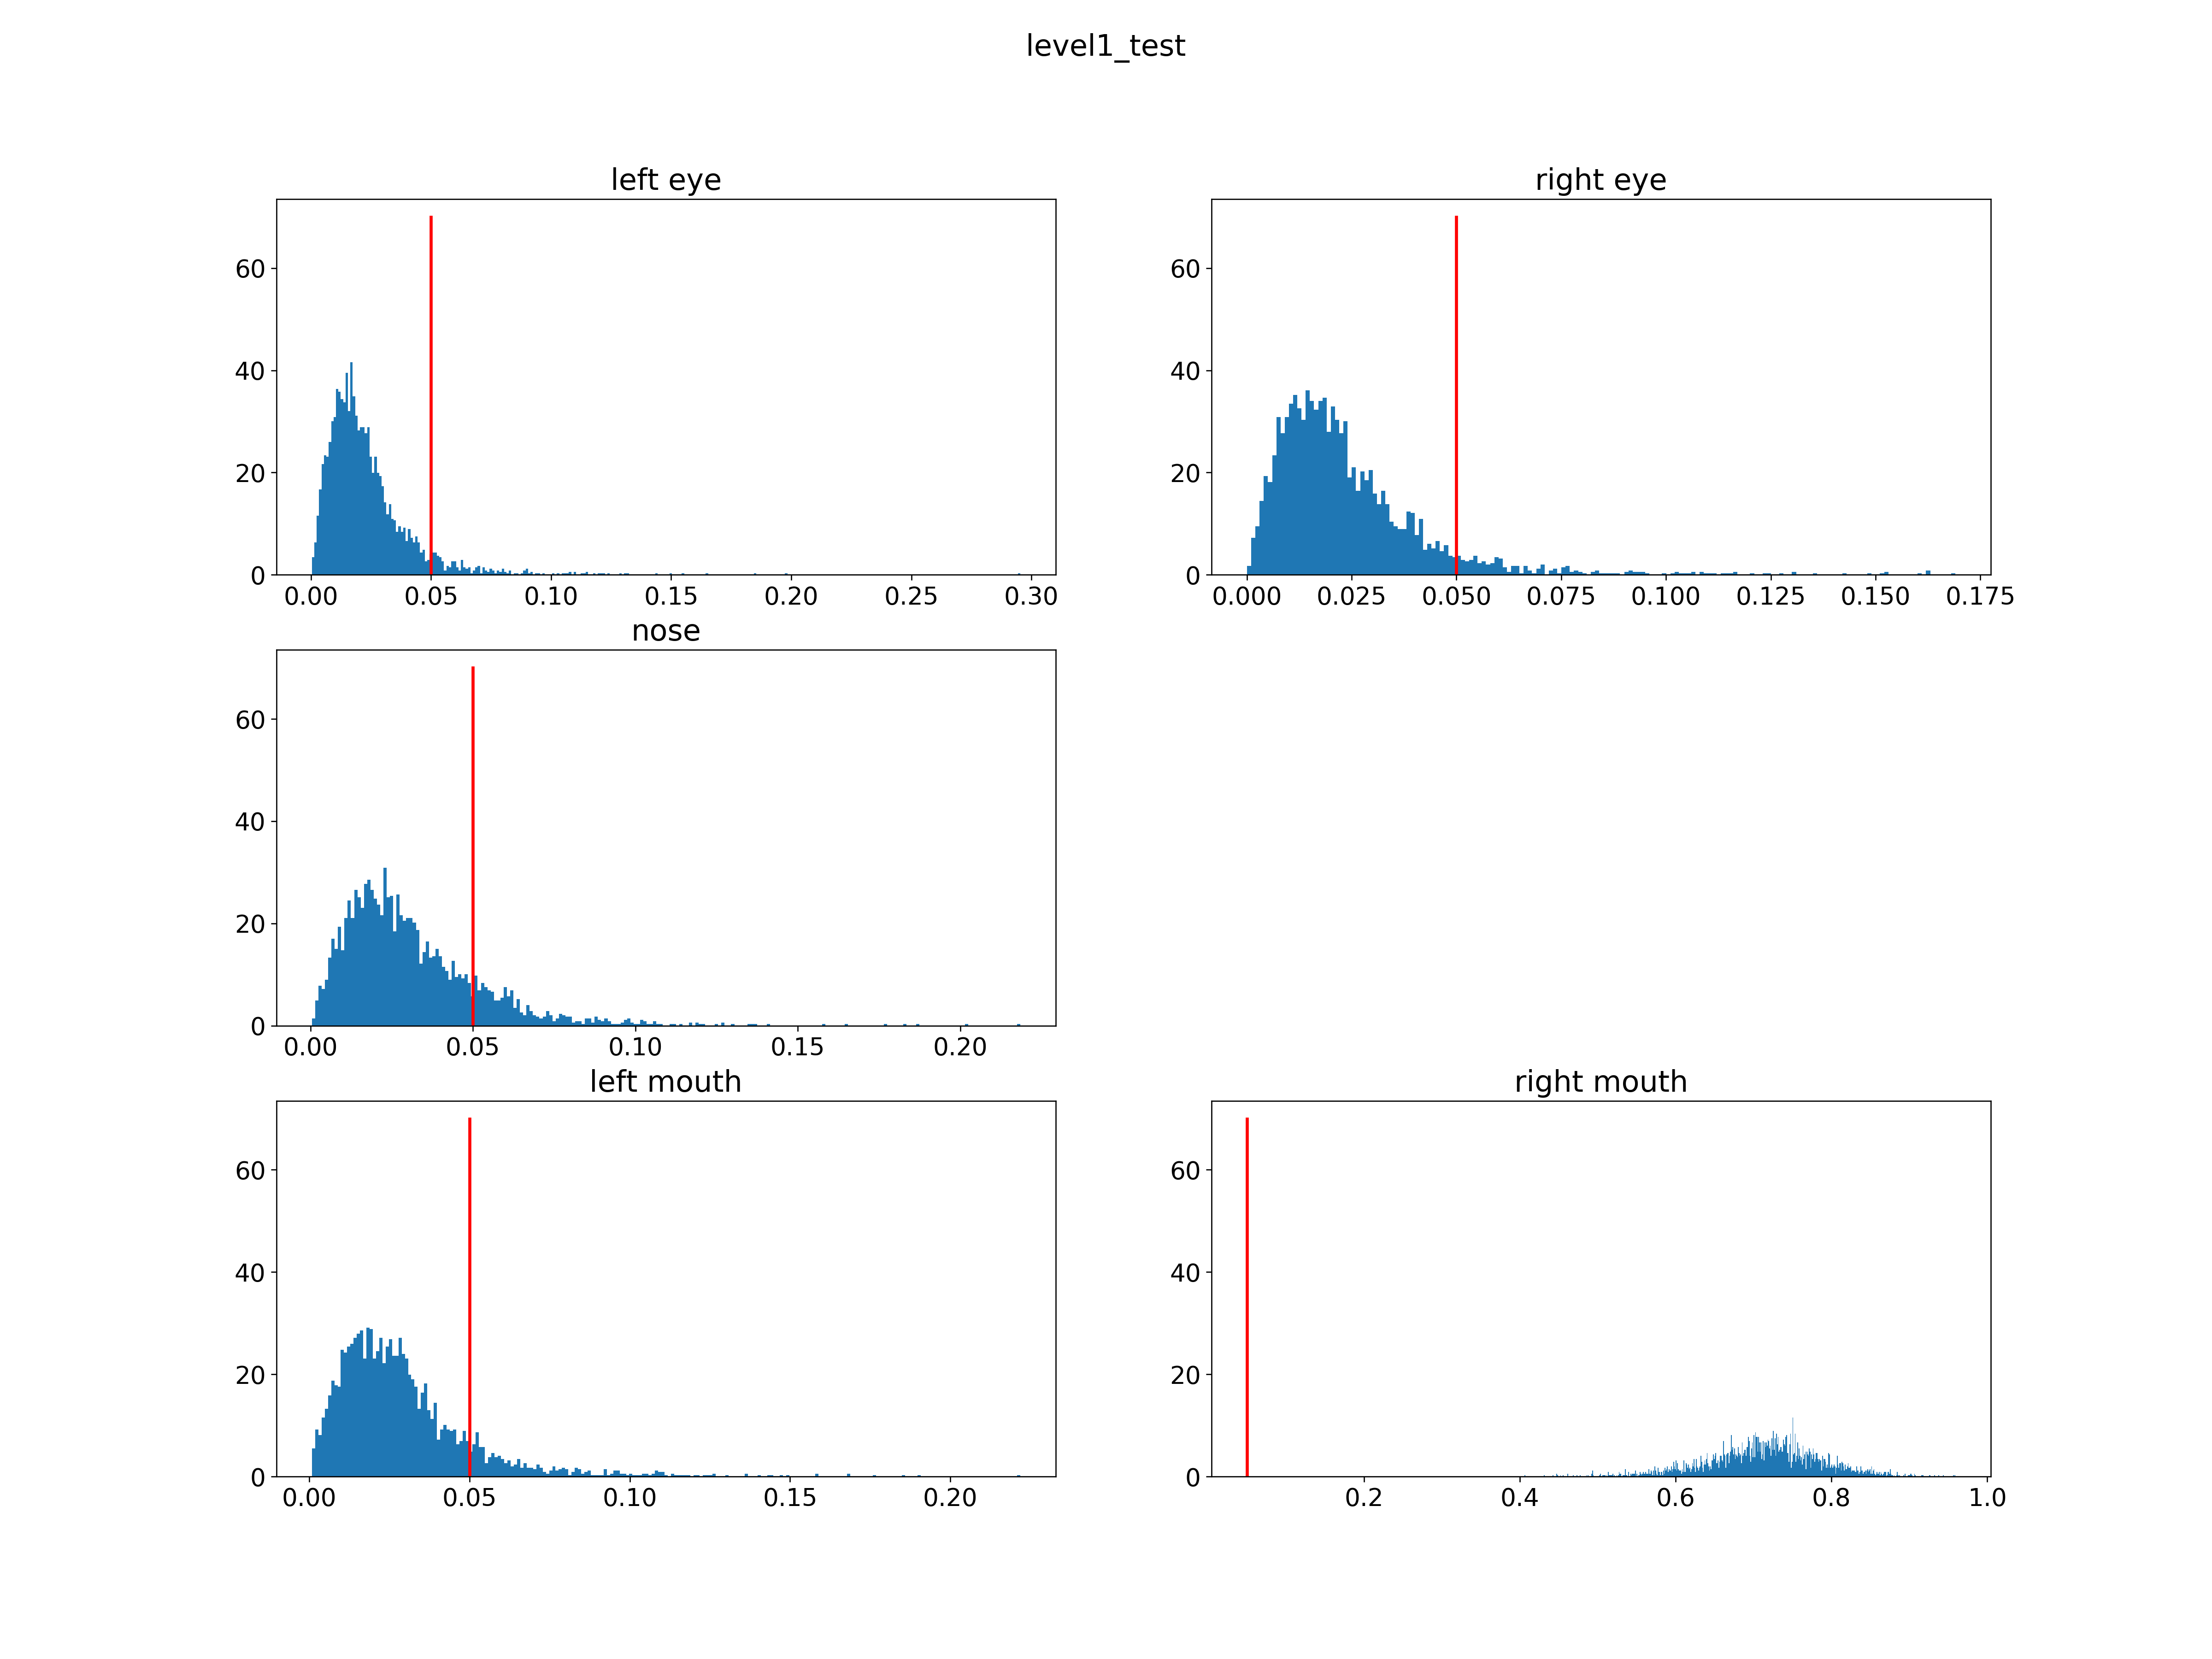
\includegraphics[scale=0.25]{images/level1_test}
	\caption{The error on each landmark in level 1}
	\label{rslevel1}
\end{figure}
\begin{figure}[h!]
	\centering
	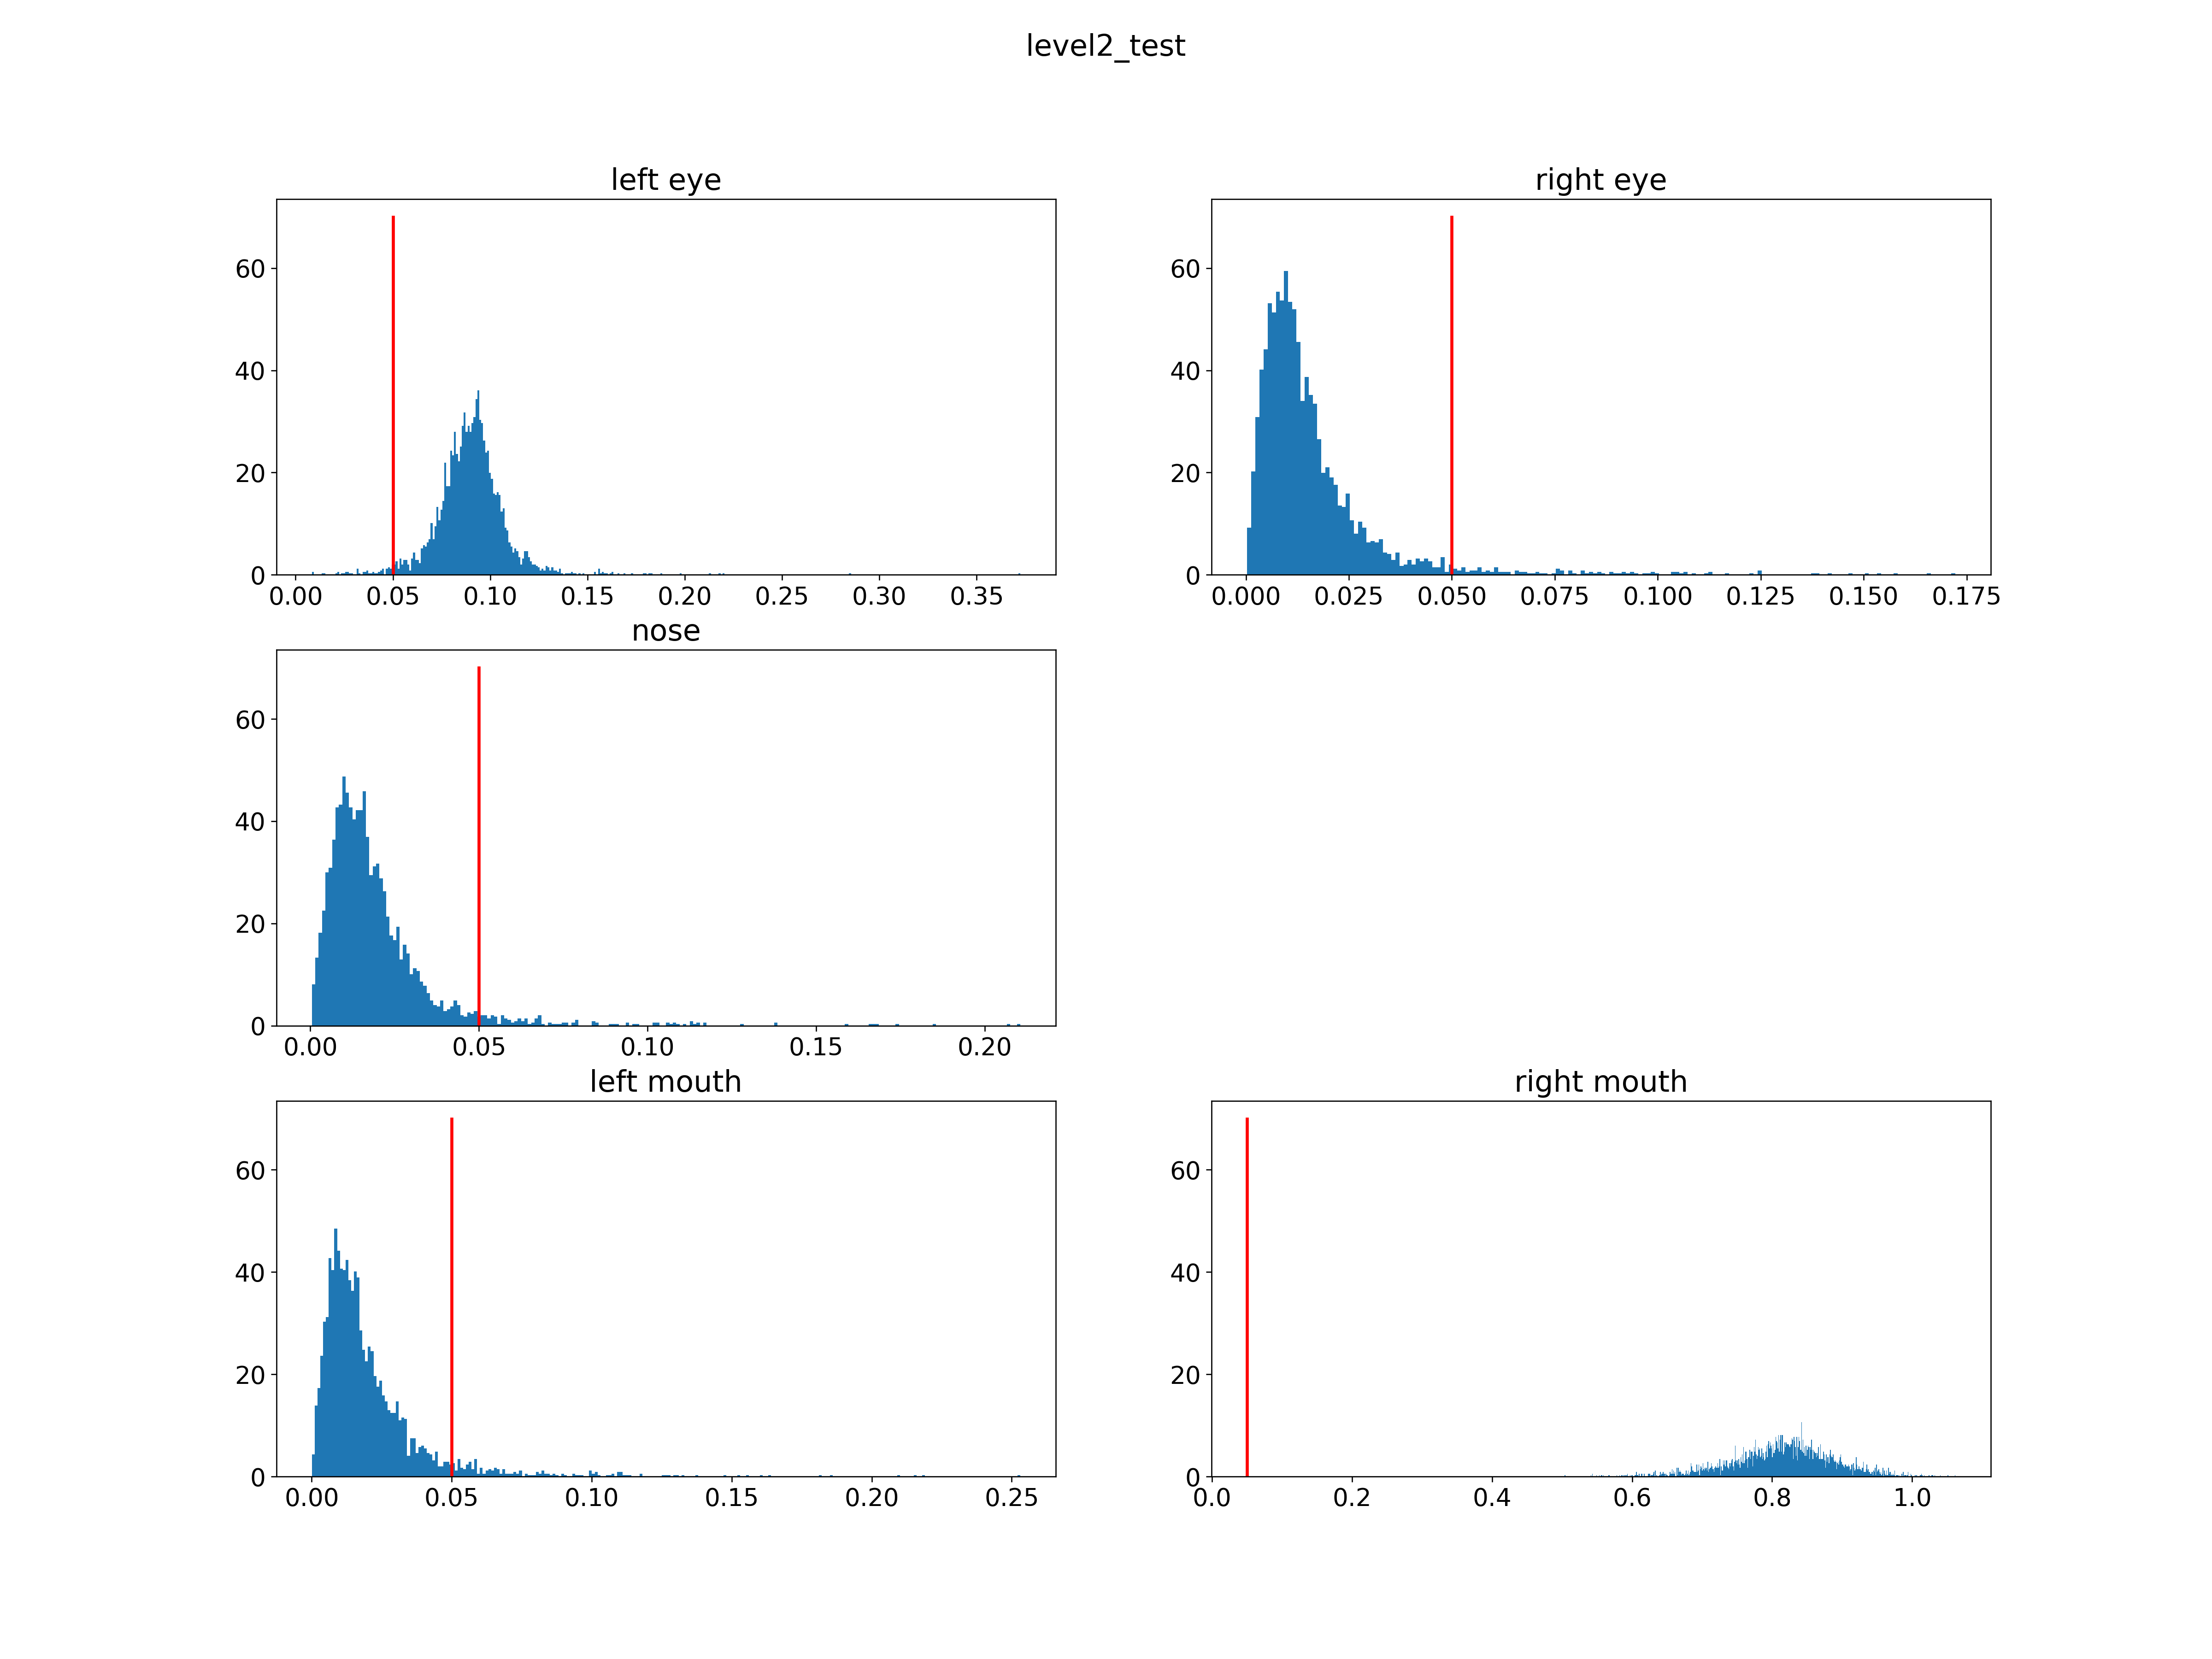
\includegraphics[scale=0.25]{images/level2_test}
	\caption{The error on each landmark in level 2}
	\label{rslevel2}
\end{figure}
	\begin{figure}[h!]
	\centering
	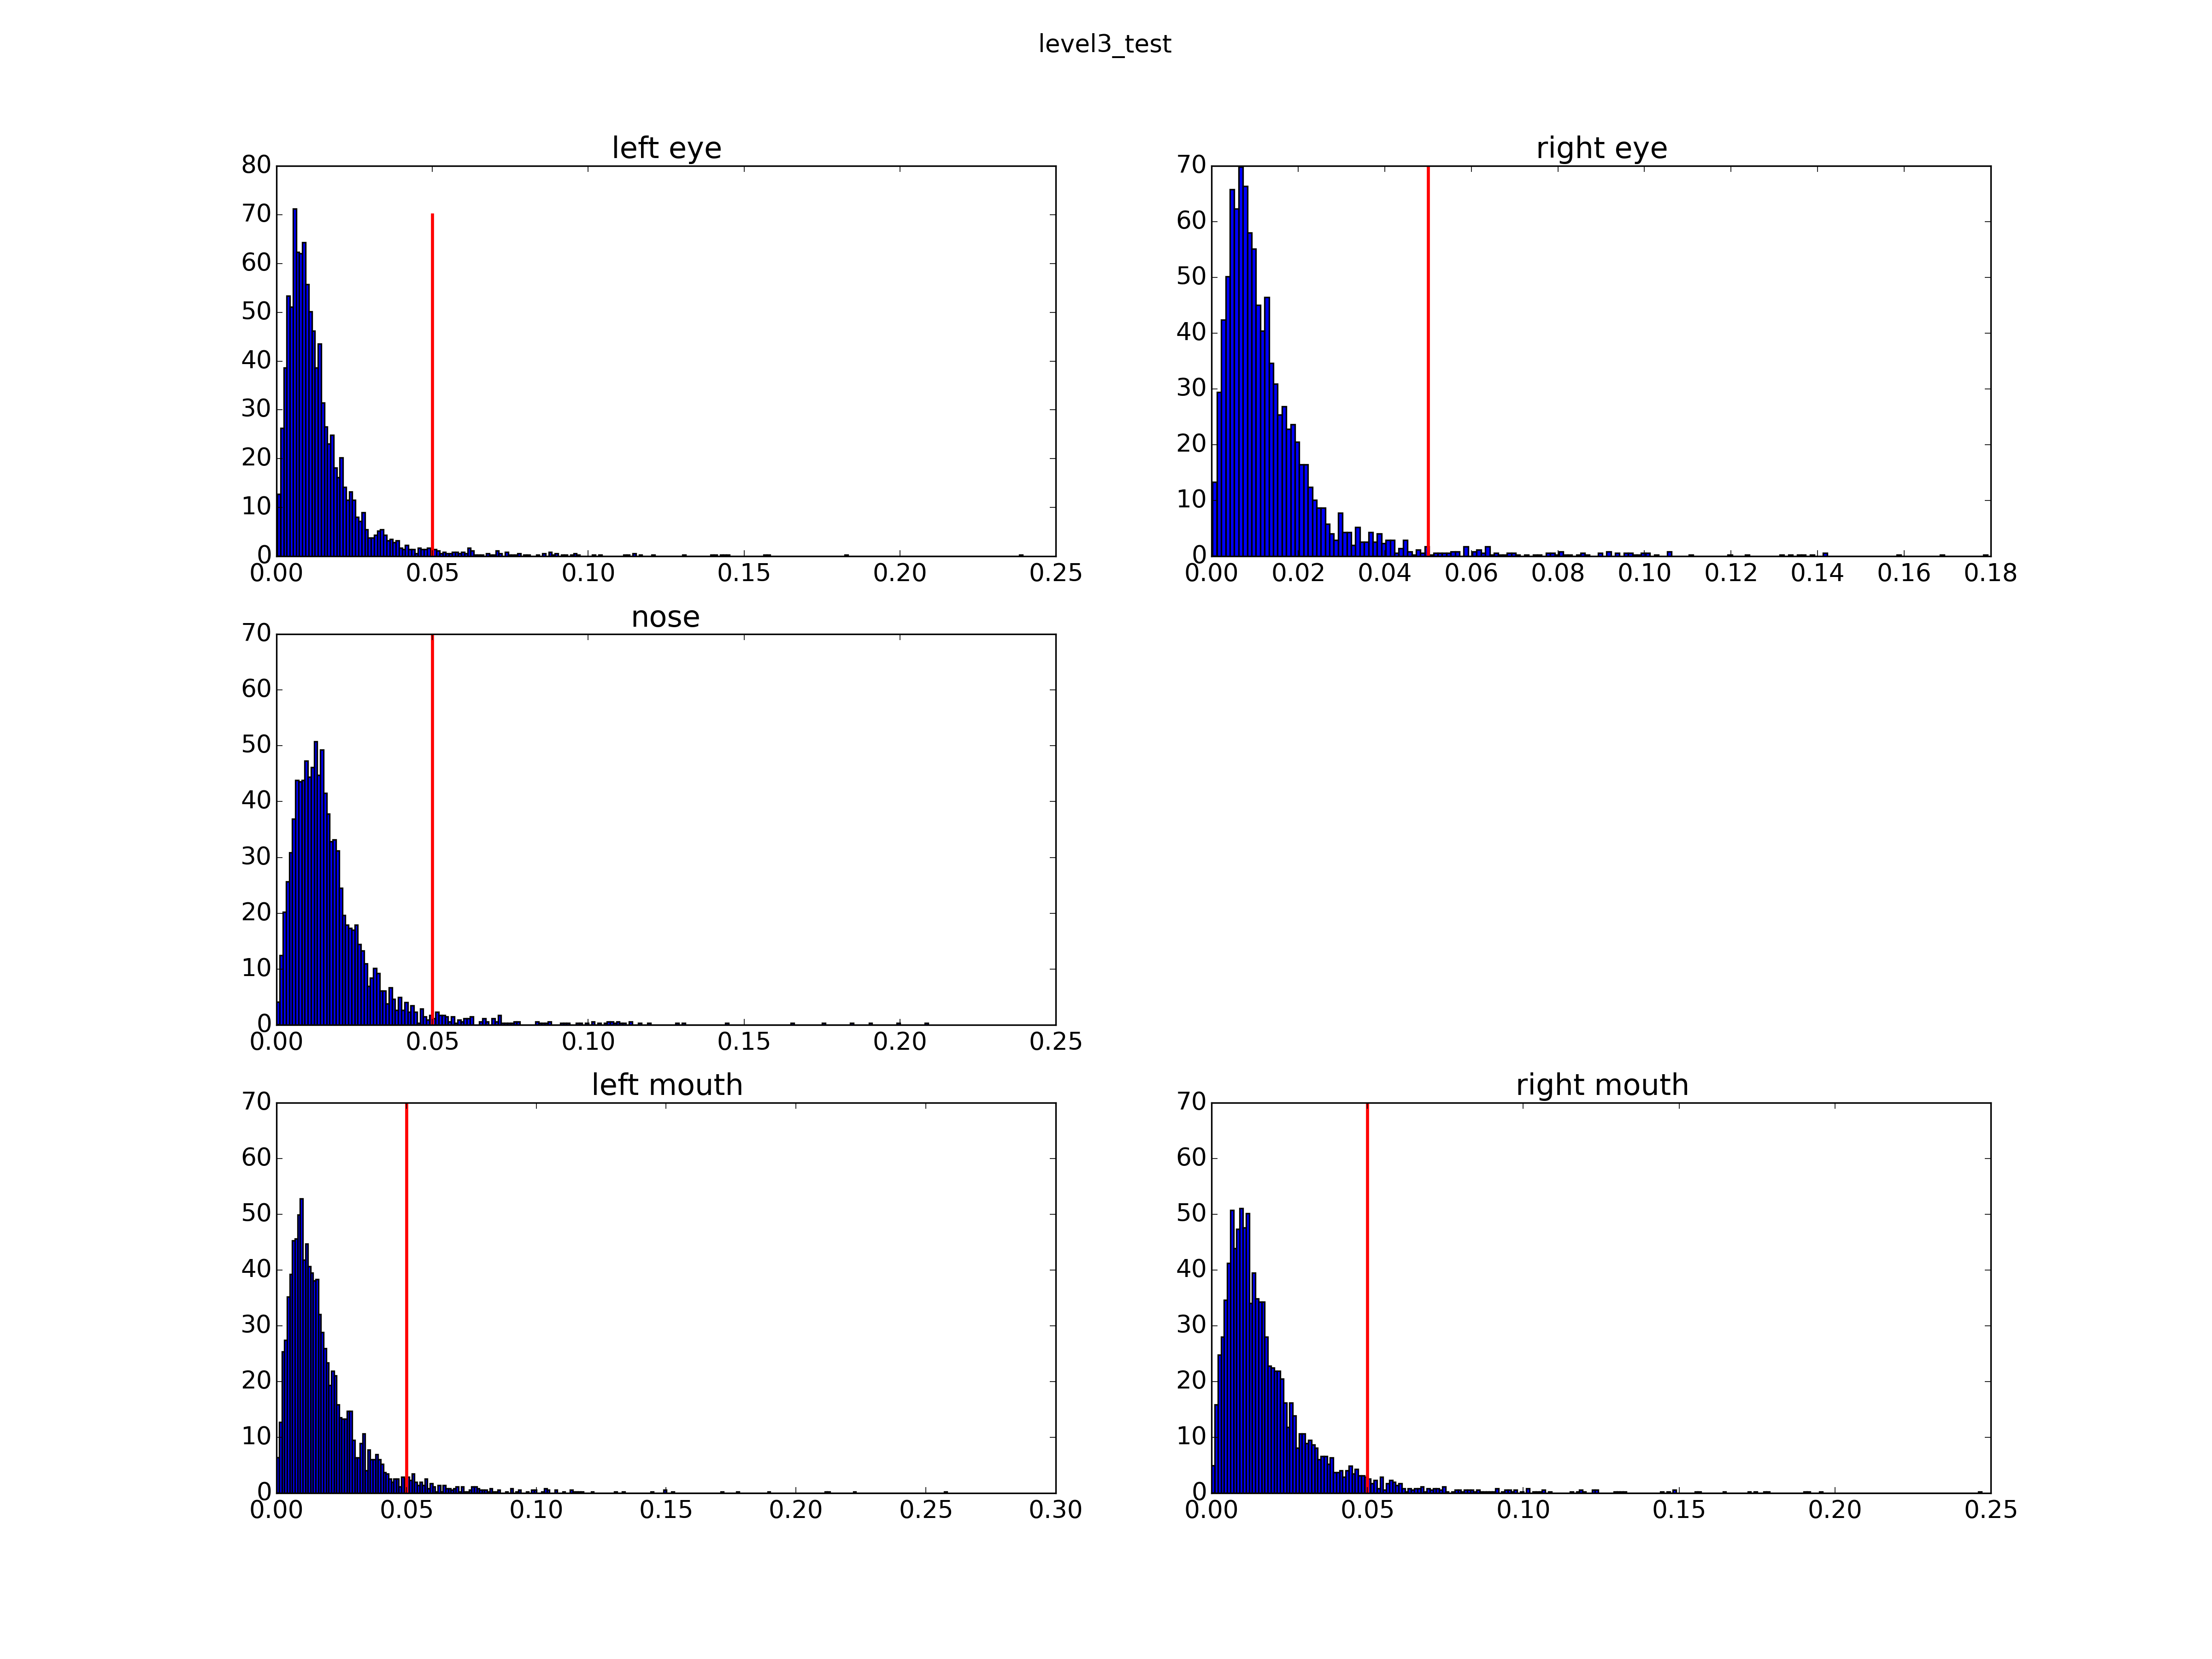
\includegraphics[scale=0.25]{images/level3_test}
	\caption{The error on each landmark in level 3}
	\label{rslevel3}
\end{figure}
\section{Model 2: Automatic ear landmarks detection by CNN}
Celia Cintas et al \cite{cintas2016automatic} proposed a method based on geometric morphometric and deep learning for automatic ear detection and feature extraction in the form of landmarks. The convolutional neural network was trained with a set of manually landmarks examples. The network is able to provide the morphometric landmarks on ear image automatically.
\subsection{Dataset}
The image and manual landmark belong to the CANDELA initiative \footnote{https://www.ucl.ac.uk/candela}, a project includes geneticists, bioinformatics and social-anthropologists interested on Latin American. CANDELA contains 7500 images with the size of $2136 \times 3216$. The provided dataset contains 2753 images which extracted from the CANDELA dataset. For each image, a set of 45 landmarks and semi-landmarks provided by human operators. The dataset was split into a training set with 2051 images (75\%) and a validation set of 684 images (25\%).
\subsection{Network}
Three models were designed and trained for performing the automatic landmarks task. These architectures are different in the number of convolution layers, the filter sizes, and the learning rate. An image with a single channel of the size  $96 \times 96$ with brightness scaled to $[0,1]$, is taken as the input of the network. The target (landmarks coordinates) is scaled to $[-1,1]$. \textbf{Fig.\ref{1Econv}} shows the best architecture. In this architecture, a structure of two convolutional layers with the filters, followed by maximum pooling and dropout layer. This structure is repeated three times to obtain features at different levels with different size of filters. After extraction the features, two fully connected linear layers with 1500 units each and a dropout layer is hired. The output layer contains 90 output units (corresponding with 45 landmarks) for the predicted position of the landmarks. The implementation used Python and the Lasagne library\cite{lasagne}.
\begin{figure}[h!]
	\centering
	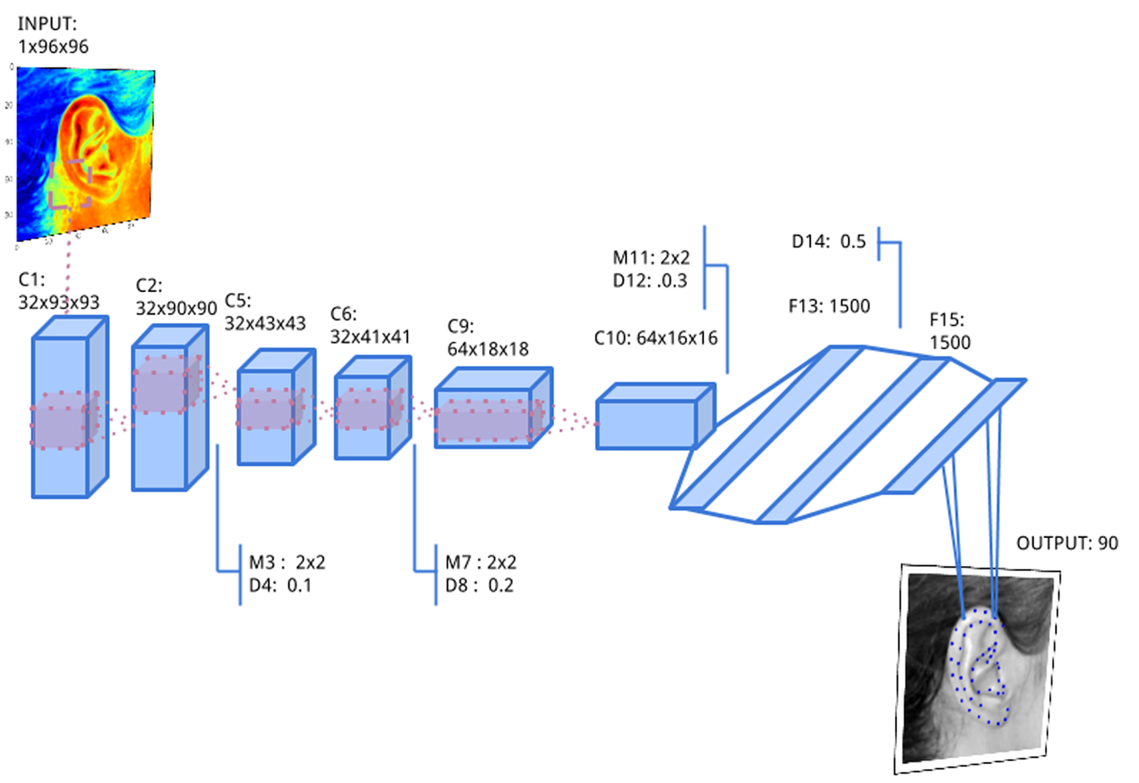
\includegraphics[scale=0.4]{images/ear_cnn}
	\caption{The best architecture for automatic ear's landmarks detection}
	\label{1Econv}
\end{figure}
\subsection{Experiments}
%Following the article, the method is evaluated the usual quality metrics for regression problems, in particular $r^2$, root mean square error (RMSE), explained variance (EV), and Pearson's correlation.
%The accuracy of three architectures are shown in Table \ref{tbear1}. Also, in Table \ref{tbear2}, the RMSE for each landmarks is shown. The regression metrics were computed using \textit{scikit-learn}\cite{}.

%\begin{table}[h!]
%	\centering
%	\begin{tabular}{l c c c}
%	& Arch0 & Arch1 & Arch2 \\ \hline
%	$r^2$ & 0.709 & 0.678 & 0.698 \\ \hline
%	RMSE & 2.296 & 2.415 & 2.338\\ \hline
%	EV & 0.976 & 0.974 &  0.975 \\ \hline
%	Pearson & 0.988 & 0.987 &  0.988 \\ \hline	
%	\end{tabular}
%	\caption{Performance of three different ConvNet architectures}
%	\label{tbear1}
%\end{table}\\
%\begin{table}[h!]
%	\centering
%	\begin{tabular}{l r}
%	\# Landmark & RMSE \\ \hline
%	1 & 1.8183 \\ \hline
%	2 & 1.2216\\ \hline
%	3 &  1.08651\\ \hline
%	4 &  1.3291\\ \hline
%	5 &  2.4477\\ \hline
%	6 &  2.59746\\ \hline
%	7 &  1.17571\\ \hline
%	\end{tabular}
%	\caption{RMS error for each landmark}
%	\label{tbear2}
%\end{table}\\

Because the CANDELA dataset is not published. Another dataset was chosen to study the network. The new dataset was used for the Facial Keypoint Detection including 7049 gray-scale images ($96 \times 96$). For each image, we are supported learn to find the position of 15 landmarks. After dropping some missing data, the dataset remains 2140 images. All the images with coordinates of manual landmarks is stored in csv file and fetched into the network. The training and validation loss are shown in Fig.\ref{earLosstrain}. The training is finished after 3000 iterations with the loss arround $10^{-3}$.
\begin{figure}[h!]
	\centering
	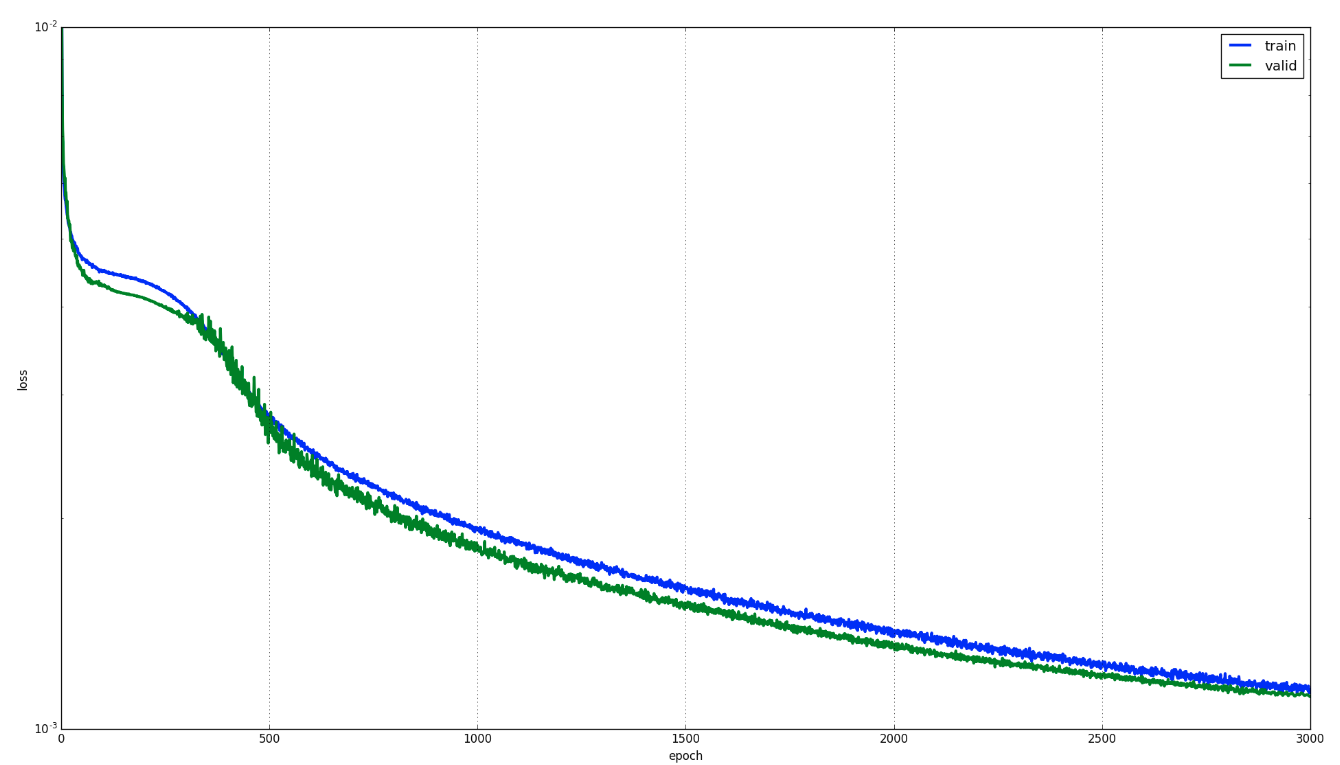
\includegraphics[scale=0.27]{images/trainloss}
	\caption{The loss of Ear-CNN network on facial point dataset}
	\label{earLosstrain}
\end{figure}
Fig.\ref{earTest} shows some test on the real facial images.
\begin{figure}[h!]
	\centering
	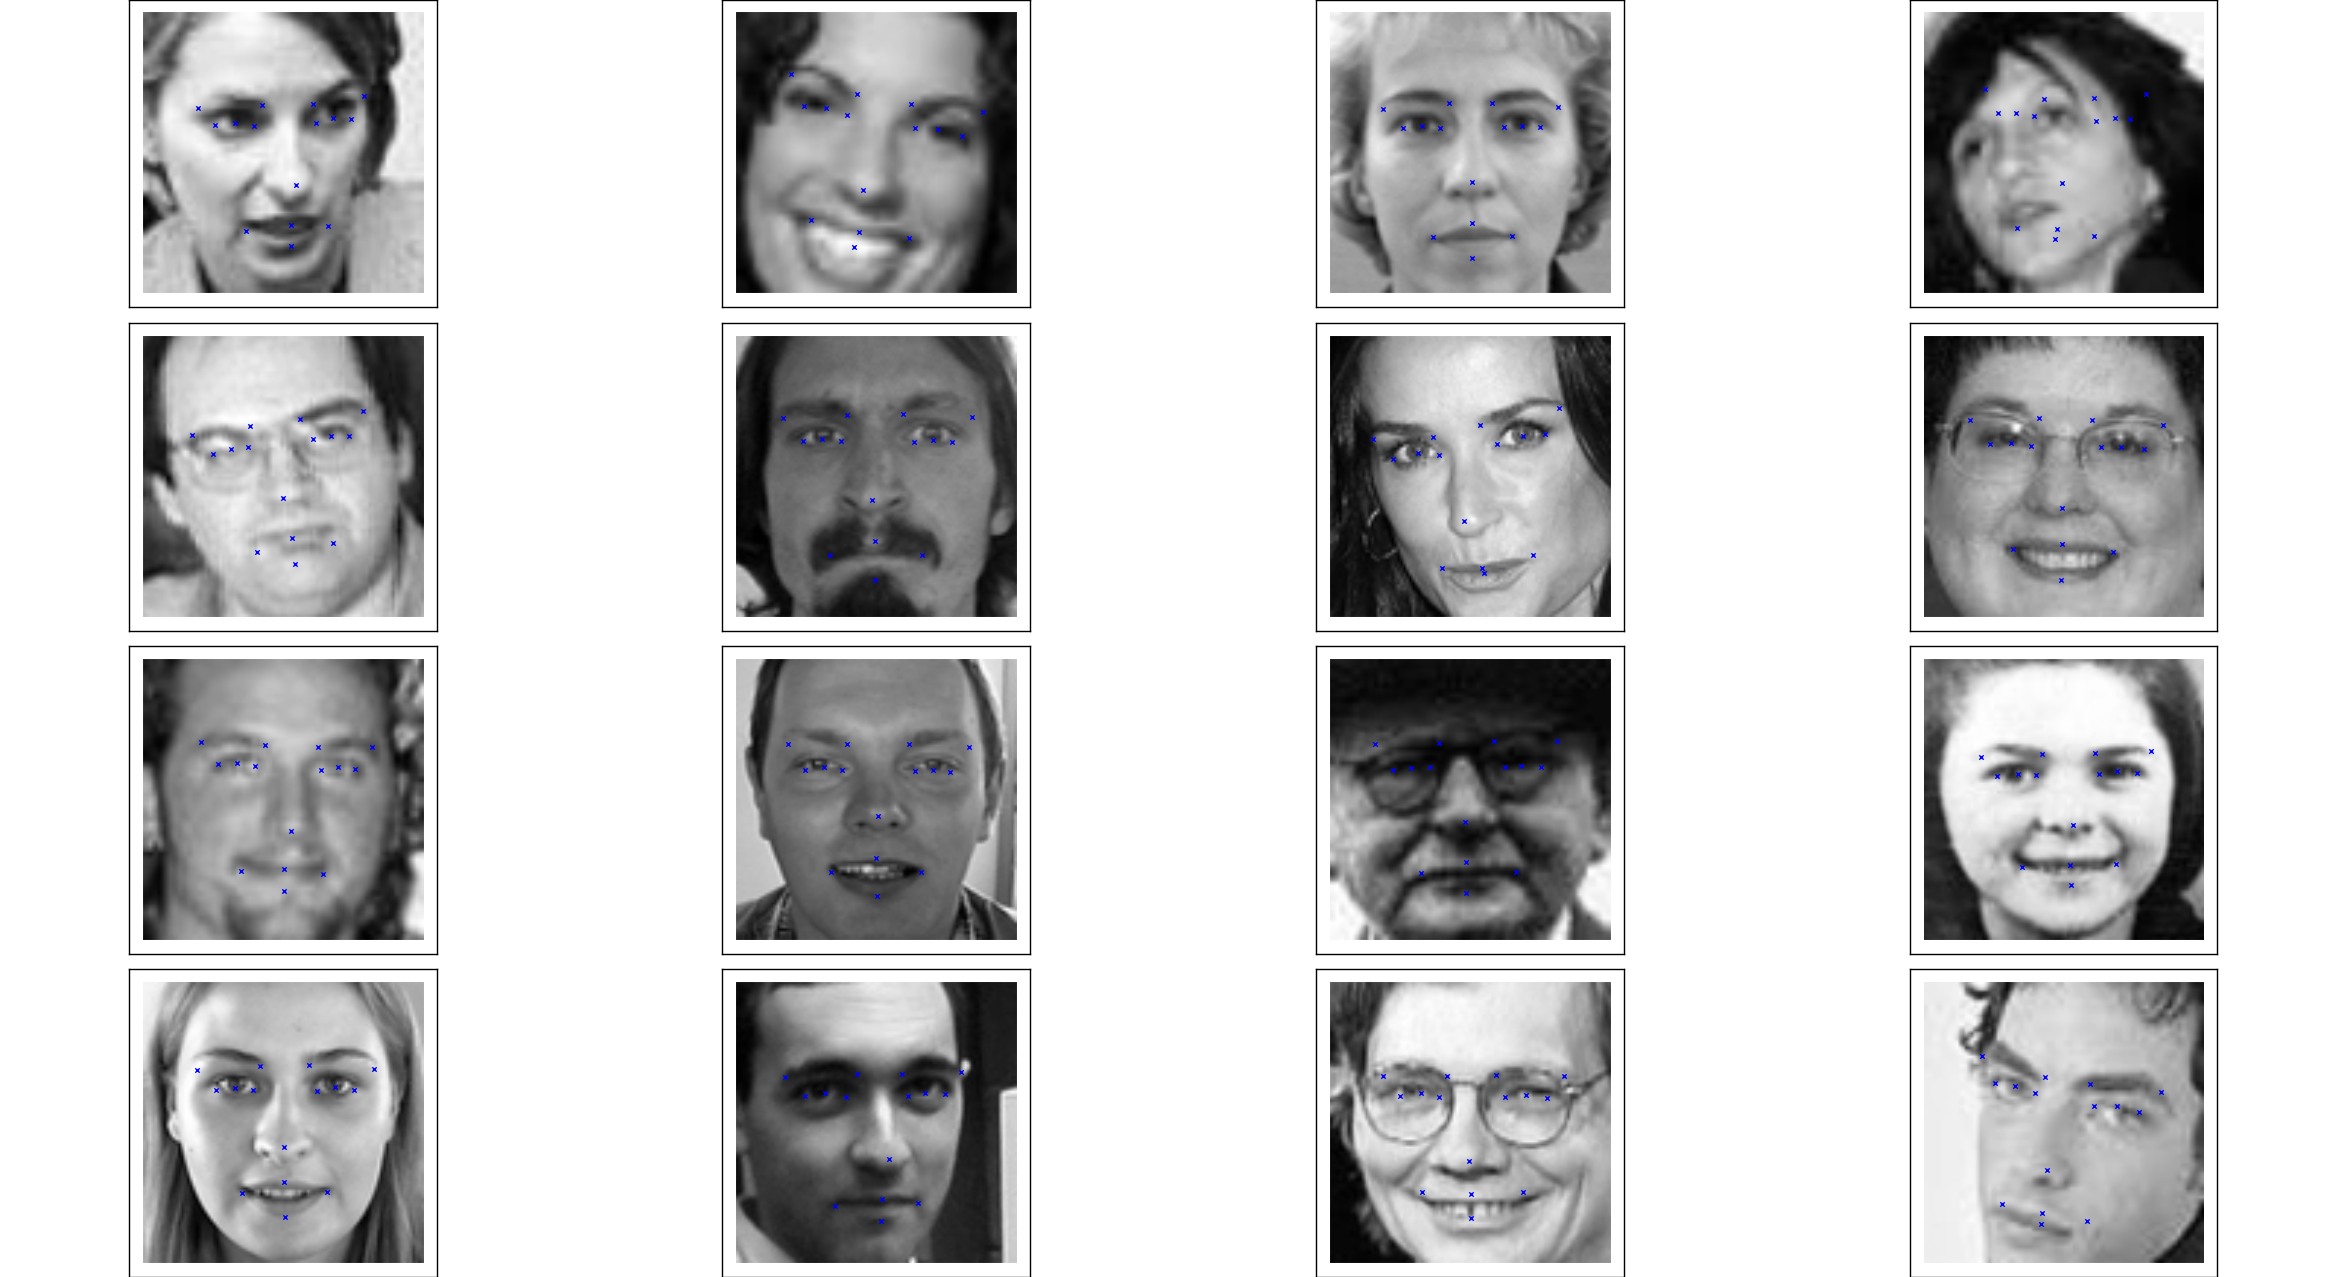
\includegraphics[scale=0.27]{images/figure_1-1.png}
	\caption{The prediction landmarks on human face}
	\label{earTest}
\end{figure}
\section{Model 1 and model 2 on pronotum}
\subsection{Dataset preparing}
The dataset includes 293 pronotum images. The images are divided into three subsets: the training set (200 images), the validation set (60 images) and the testing set (33 images). Because the dataset is limited and the models are worked on gray-scale images, we applied some ways to en-large the dataset. Firstly, for each original image in RGB, each channel is modified by adding some values. Secondly, the channels of the original image are split. So, we have obtained 1600 images for the training set and 480 images for the validation set. At the end, the images are down-sampled with the  size of $256 \times 192$ before giving to the networks.

%To enlarge the dataset during training, the image in training and validation set are augmentation by modifying the valued of red and green channel. So, at the end, we have 600 and 180 images in training and validation set, respectively.
\subsection{Model 1 and pronotum landmarks}
The networks in the first level are modified to suitable with the prediction of landmarks on the pronotum (8-landmarks). For each pronotum, eight manual landmarks have been set. The bounding box is created depending on the coordinate of the manual landmark. The networks in the first level are used as followed:
\begin{itemize}
	\item F1 network recognizes whole pronotum bounding box with eight landmarks.
	\item EN1 network predicts the location of the first five-landmarks.
	\item NM1 network is used to estimated the position of last four-landmarks and the first landmark.
	\item At the end, the position of each landmark is average of the predicted position in the networks.
\end{itemize} 
\subsubsection{Testing}
The error rate of each network during training is shown in the Table.\ref{model1p}:\\
\begin{table}[h!]
	\centering
	\begin{tabular}{l r}
	Network & Loss \\ \hline
	F1 & 0.013 \\ \hline
	EN1 & 0.47\\ \hline
	NM1 &  0.5
	\end{tabular}
	\caption{The loss of the networks in Model 1 on pronotum dataset}
	\label{model1p}
\end{table}
\begin{figure}[h!]
\centering
\subfloat[Test 1]{\label{}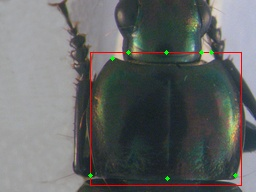
\includegraphics[width=0.2\textwidth]{./images/test1}}~~
\subfloat[Test 2]{\label{}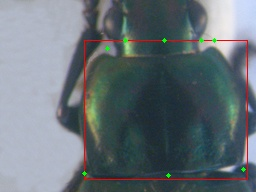
\includegraphics[width=0.2\textwidth]{./images/test2}}\\
\subfloat[Test 3]{\label{}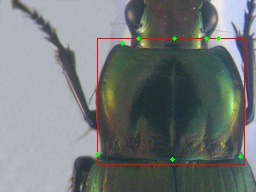
\includegraphics[width=0.2\textwidth]{./images/test3}}~~
\subfloat[Test 4]{\label{}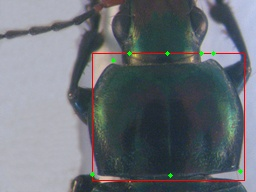
\includegraphics[width=0.2\textwidth]{./images/test4}}\\
\caption{The pronotum with predicted landmarks at level 1}
\label{model1pTest}
\end{figure}\\
From the result, the errors of EN1 and NM1 still high. That errors make the prediction result of level 1 do not enough good. Besides, the networks at level 2 and level 3 used the prediction at level 1 as the input data to predict the new position. So, we can not continue with the level 2, 3 until the result at level 1 is improved. Perhaps, the model in model 1 is not suitable to detect the landmarks on pronotum.  Fig. \ref{model1pTest} shows the prediction landmarks on four images. Followed that, the networks can be detected the landmarks at position 4, 5 and 7; the different position still not good.
\subsection{Model 2 and pronotum landmarks}
The dataset is kept the same with model 1 (2080 images) but having some changes. Firstly, the ways to choose the data(to train and validate) is changed. All images are combined. Then, the network will automatically choose $75 \%$ data to train and $25 \%$ for validation. Secondly, the inputs that given to the network are just the image and landmarks(without the coordinate of the bounding box).

The network is run 3000 iterations with the learning rate begin from $0.08$ to $0.01$. During training, the learning rate is changed to fit with the remaining iterations\cite{lecun2012efficient}. Fig.\ref{model2pl} shows the first 700 iterations during training. The loss did not have many changes after $100^{th}$ iteration.

\begin{figure}[h!]
	\centering
	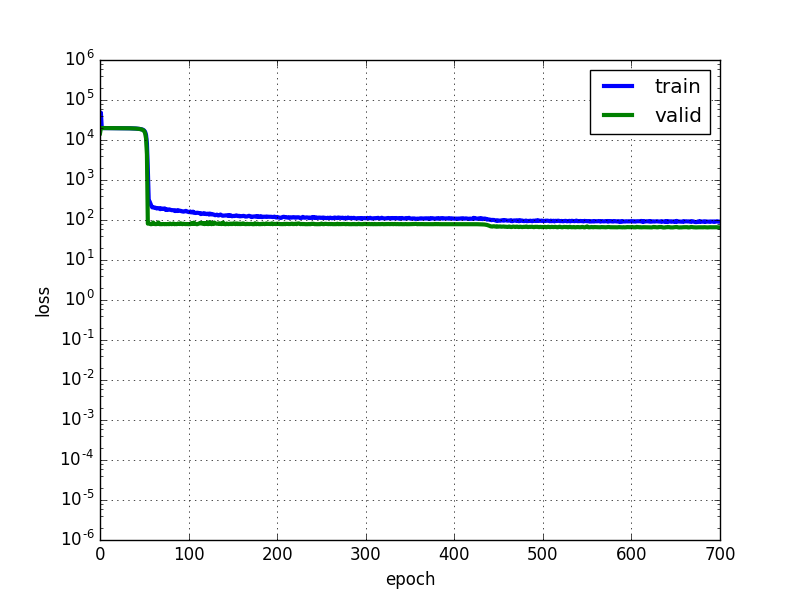
\includegraphics[scale=0.4]{images/figure_1_loss_celia}
	\caption{The losses of model 2 on pronotum dataset}
	\label{model2pl}
\end{figure}

\begin{figure}[h!]
	\centering
	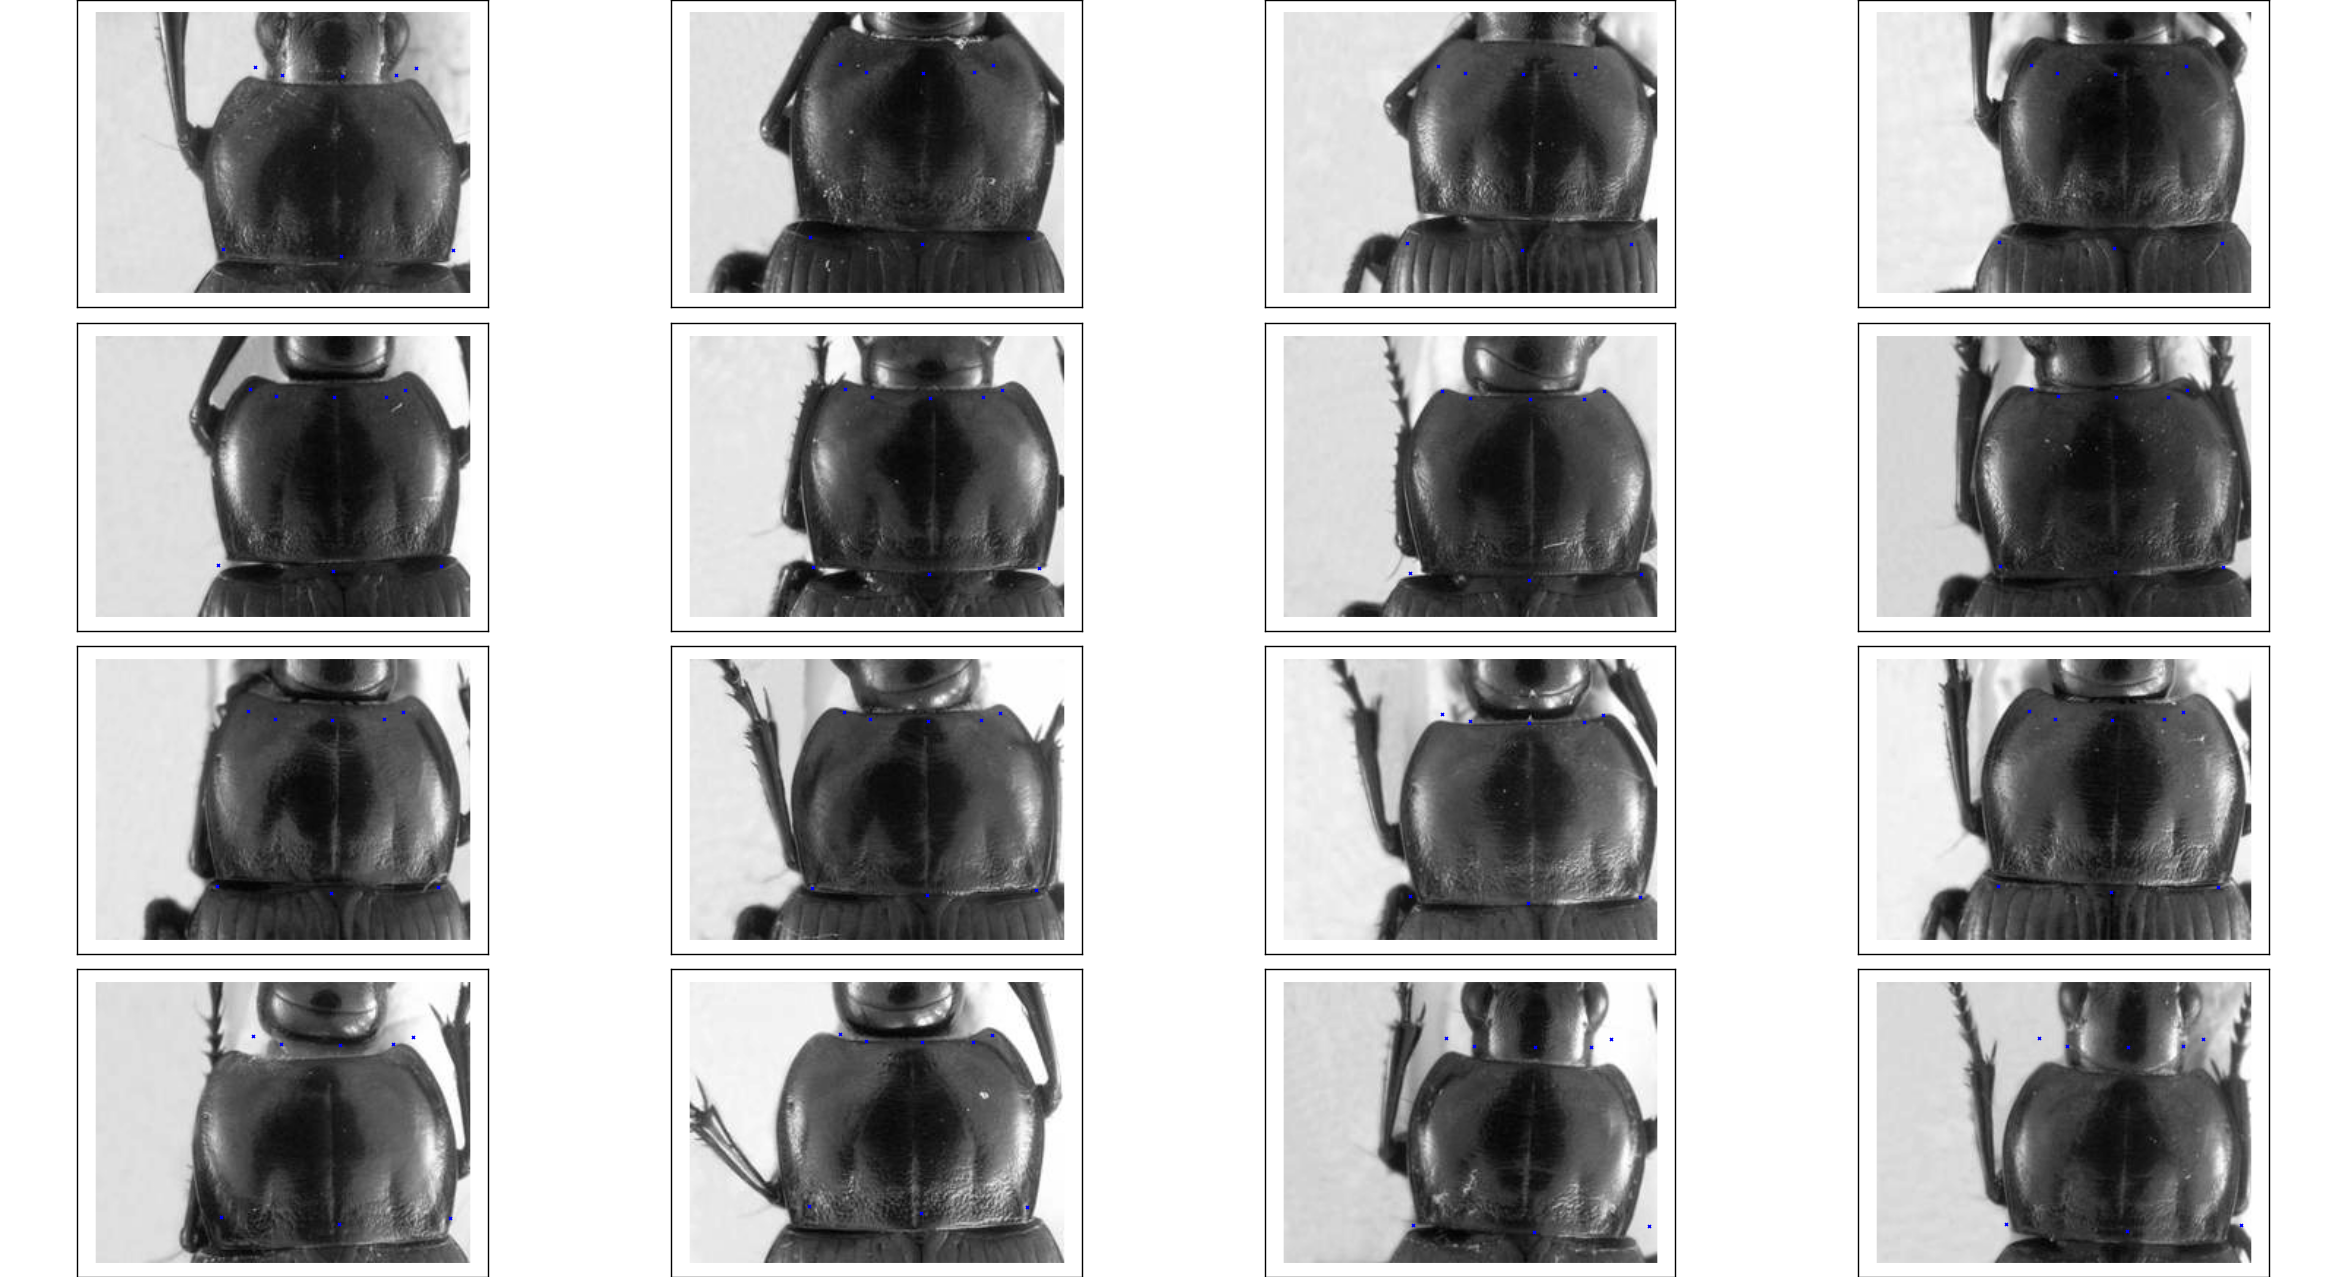
\includegraphics[scale=0.25]{images/figure_1_celia}
	\caption{The prediction landmarks on pronotum of model 2}
	\label{model2pt}
\end{figure}
Fig.\ref{model2pt} shows the prediction landmarks on 16 images. Following, the prediction landmarks from the network of model 2 are closed with the pronotum but the location is still inaccurate.

%\subsection{Comparing model 1 and model 2}
%Table C shows some differences from 2 models
%\begin{table}[h!]
%	\centering
%	\begin{tabular}{l c c c}
%	Model & Framework & Dataset (images) & Learning rate \\ \hline
%	Model 1 & Caffe & 13466 & 0.013 \\ \hline
%	Model 2 & Lasagne(Theano) & 2140 & zz\\
%	\end{tabular}
%\end{table}\\
\section{Proposed architecture}
\subsection{Model and parameters}
From the tutorial of Daniel Nouri\footnote{http://danielnouri.org/} about using CNN to detect facial key points. We propose a CNN to detect the landmarks on pronotum. The proposed network includes three convolutional layers followed by three maximum pooling layers and three full connected layers(Fig.\ref{pmodel}). The network receives the gray-scale image ($256 \times 192$) as the input. The deep of convolutional layers is increased from $32, 64, $ and $ 128$ with different size of filter while we keep the same size of filter for pooling layers. At the end of the network, three full-connected layers with the size of $500, 500, $ and $16$ are set up to predict the landmarks. Besides, the model is designed with a small sharing learning-rate and the momentum. The learning-rate and the momentum are changed overtime of training.
\begin{figure}[h!]
	\centering
	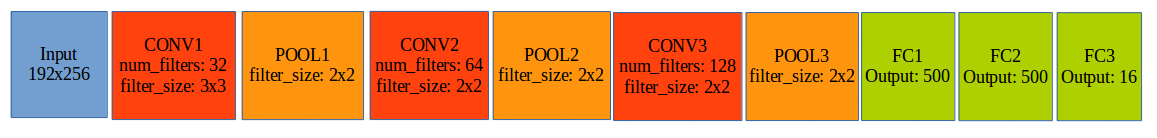
\includegraphics[scale=0.4]{images/proposed_model}
	\caption{The architecture of proposed model}
	\label{pmodel}
\end{figure}
\subsection{Training and experiments}
The model is trained with 2080 images(mentioned before) in 3000 iterations. The images are normalized before giving to the network by scaling the intensity value to [0,1], instead of 0 to 255. The target values (x and y coordinates) is kept as original. During the training, the root-mean-square error (MSE) is used to calculate the loss.
\begin{figure}[h!]
	\centering
	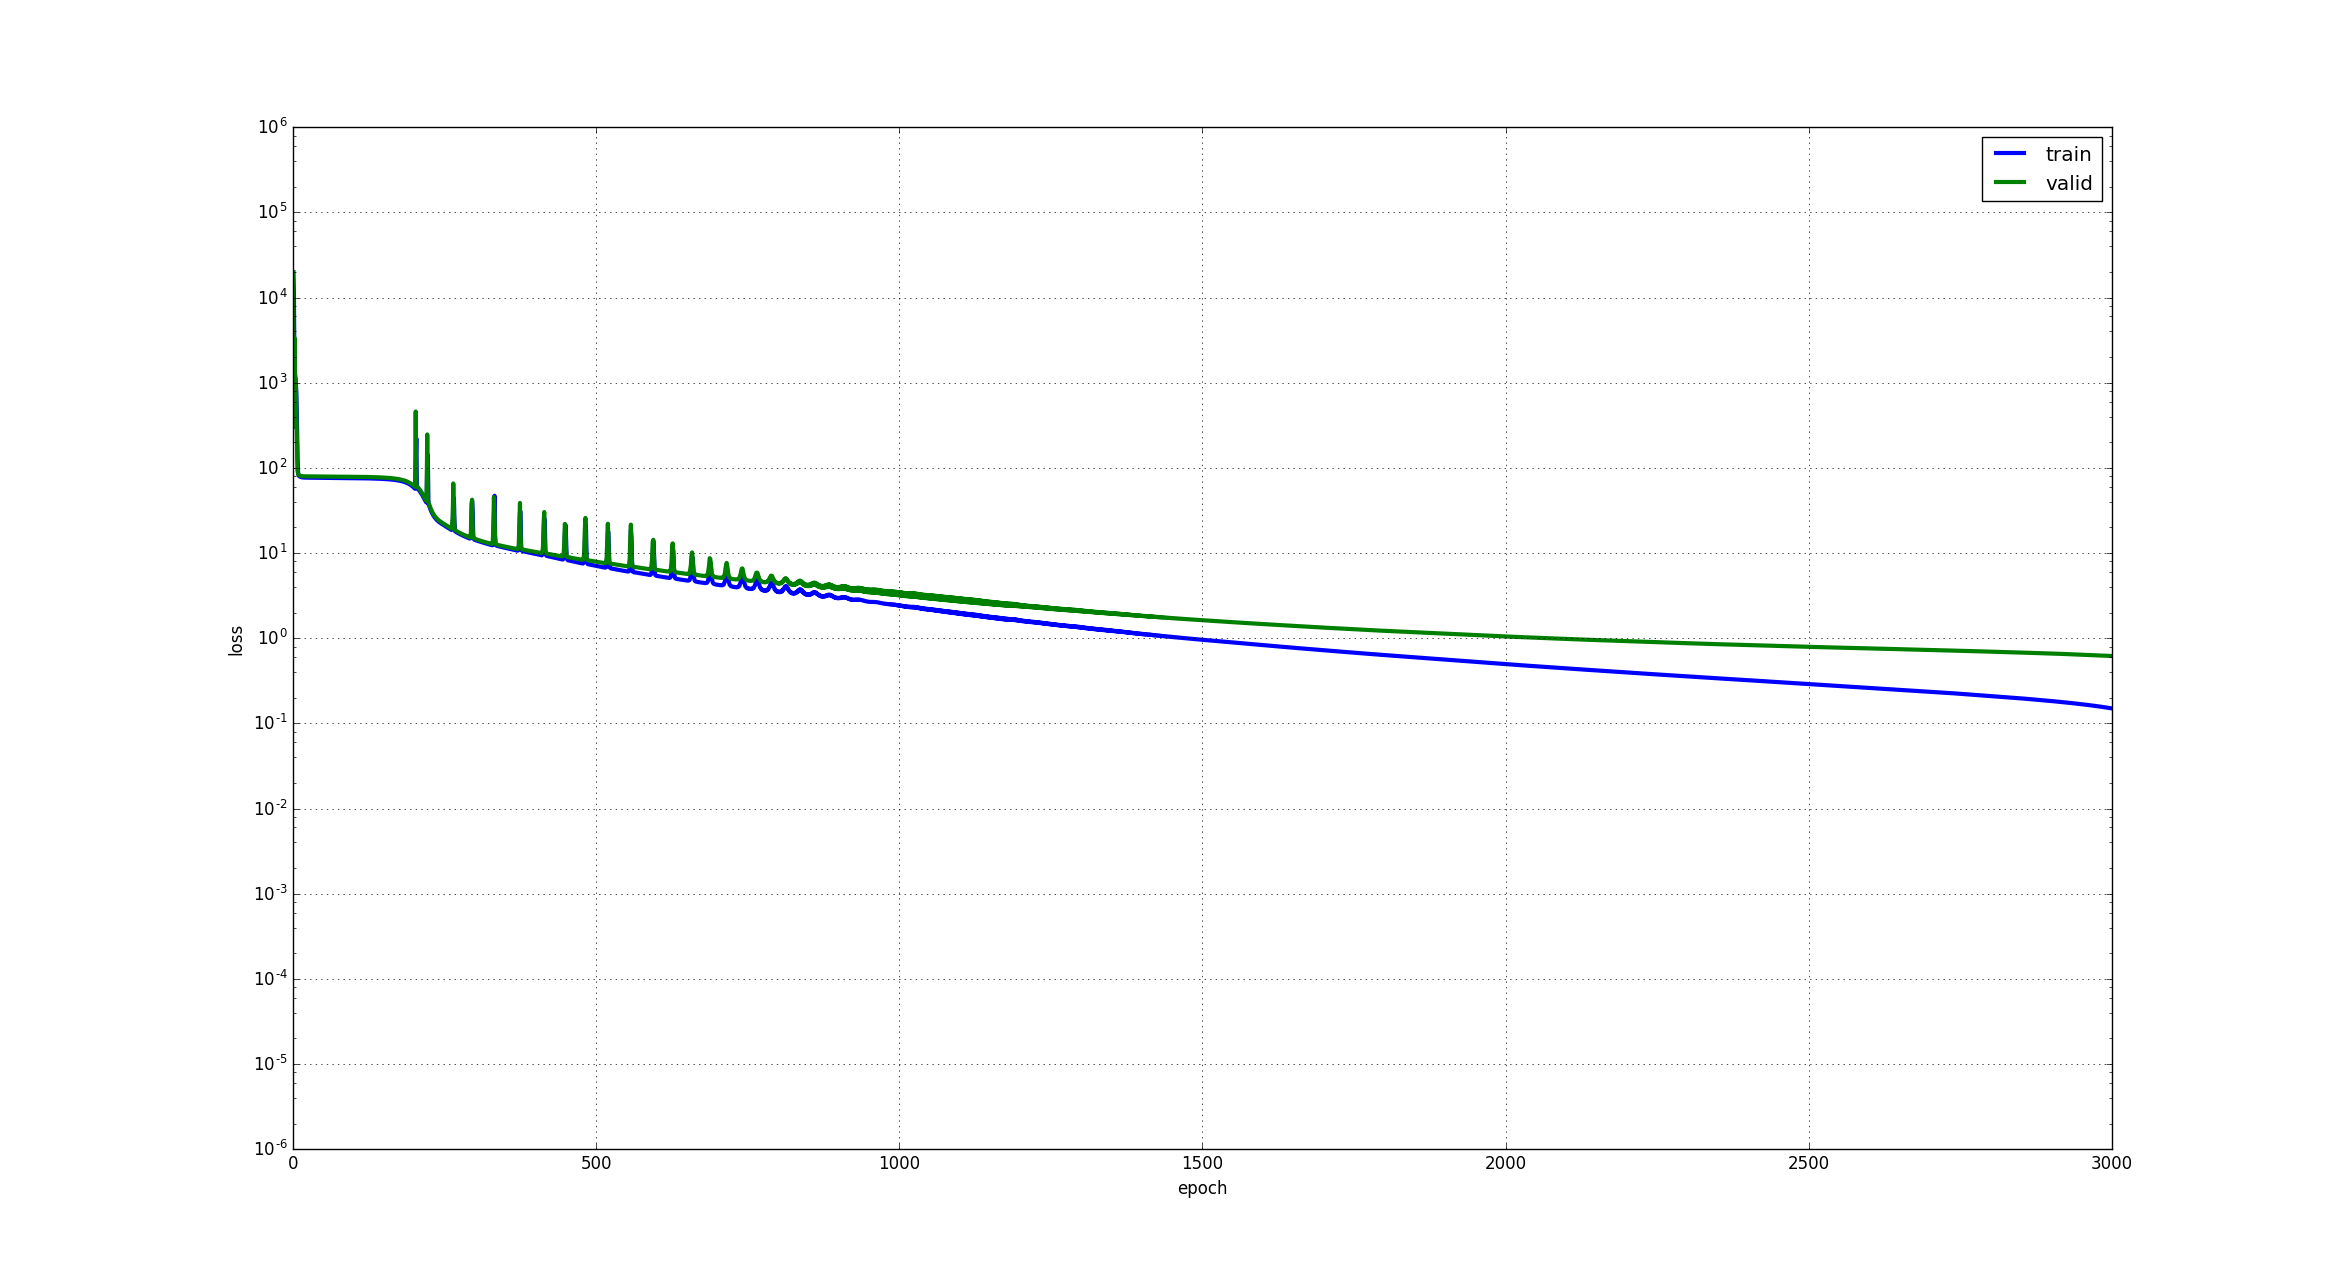
\includegraphics[scale=0.25]{images/figure_1_loss_cnn3_3000_2}
	\caption{The loss during training and validation}
	\label{cnn3l}
\end{figure}

Fig.\ref{cnn3l} shows the loss of training and validation. We can see that, at the first 200 iterations, the loss is not changed. When the training is longer and the learning rate is improved, the loss is decreased and a large distance between training and validation is appeared (over-fitting) but it is not that bad. With the loss of $0.1$ by MSE, the model is enough good to predict the landmark on pronotum. Fig.\ref{cnn3t}, Fig.\ref{cnn3t1} show the location of prediction landmarks on test dataset.
\begin{figure}[h!]
	\centering
	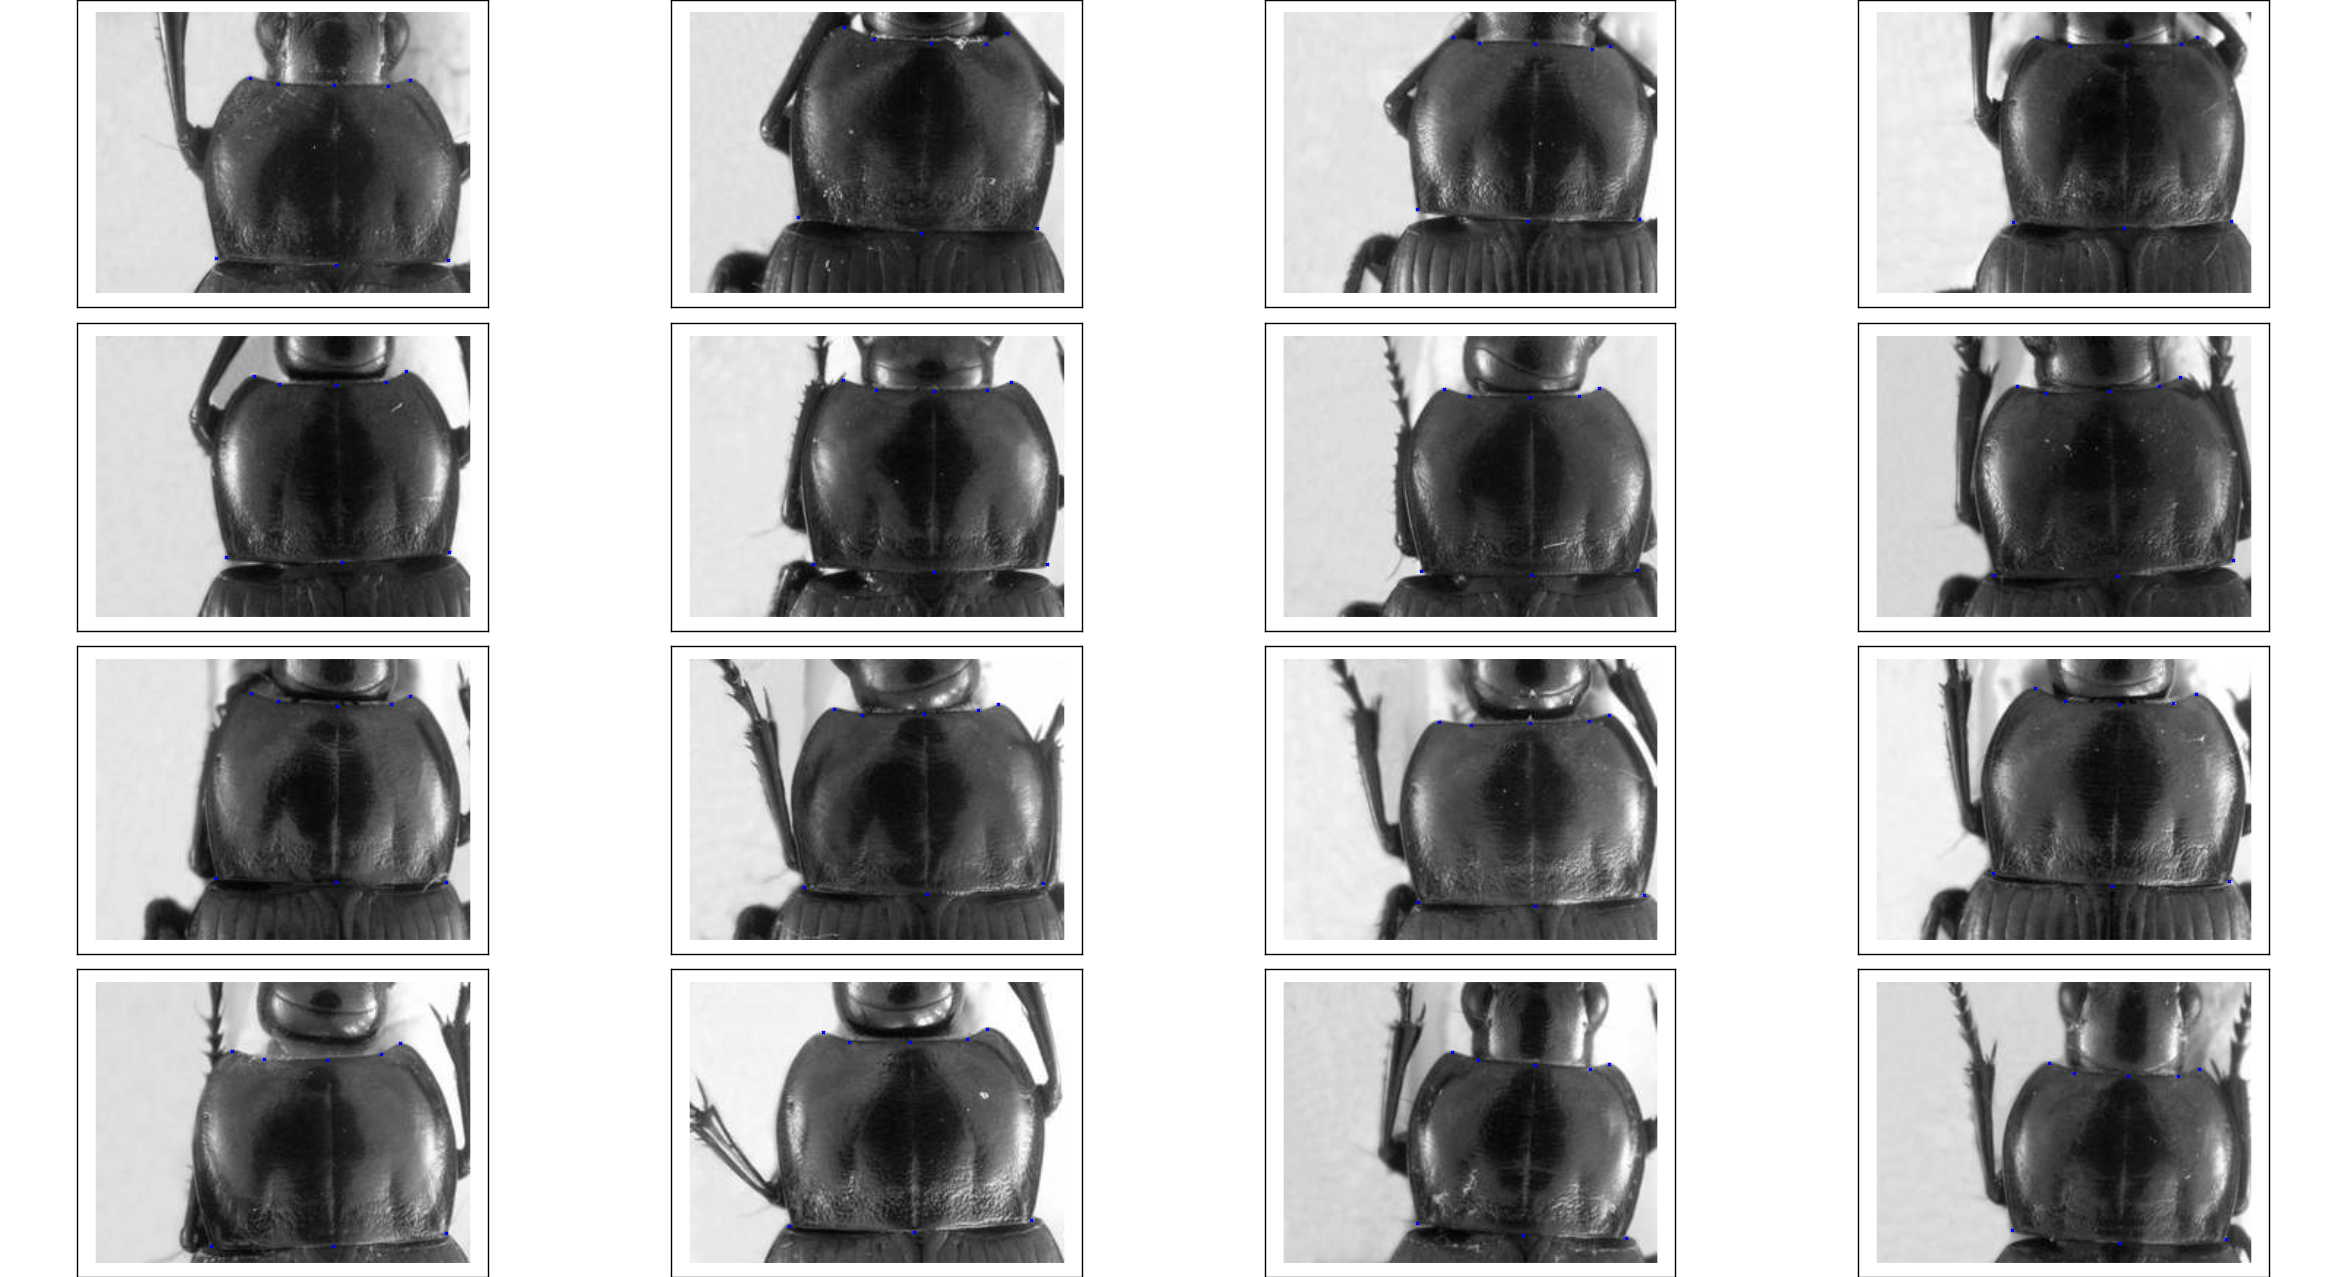
\includegraphics[scale=0.3]{images/figure_1_cnn3_3000_2}
	\caption{The prediction landmarks on 16-pronotum images}
	\label{cnn3t}
\end{figure}
\begin{figure}[h!]
	\centering
	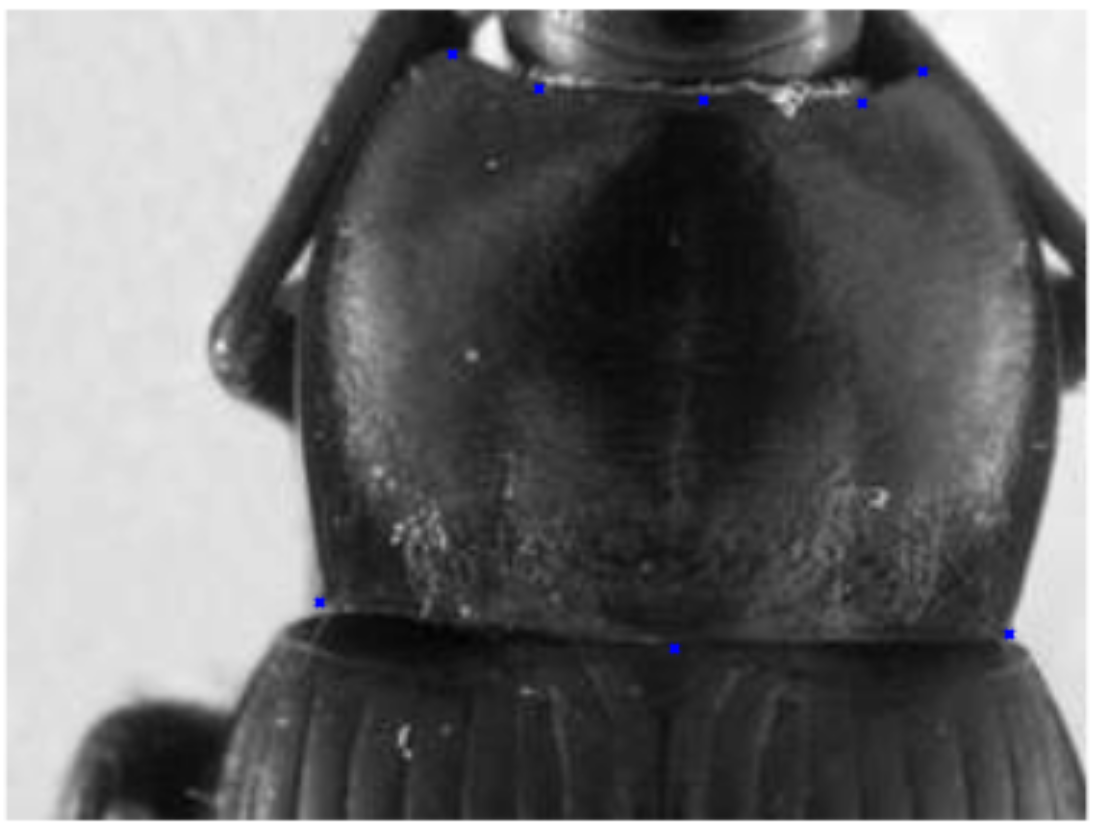
\includegraphics[scale=0.3]{images/plandmark}
	\caption{The prediction landmarks on a pronotum}
	\label{cnn3t1}
\end{figure}
\section{Conclusions}
In this chapter, we have studied two methods to predict the landmarks on 2D gray-scale images. For each case, the model is suitable with different dataset but the results are still not good when we change the data (pronotum). Besides, we proposed a network to learn and detect the landmark positions on pronotum. The accuracy of the model is greater than $98 \%$ and we believe that the network is enough good to predict the landmark on pronotum dataset.
\bibliographystyle{unsrt}
\bibliography{includes/references}
\end{document}